%-------------------------------------------------------------------------------
\chapter{Numerical Results}\label{cap5} 
\vspace{-1cm} \vspace{1cm}

%\begin{flushright}
%\begin{minipage}{0.7\linewidth}
%\emph{``O homem � como uma fun��o, cujo numerador � o que ele � e
%cujo denominador � o que ele pensa dele mesmo. Quanto maior o
%denominador, menor a fra��o.''}
%\end{minipage}
%\end{flushright}
%
%\begin{flushright}
%{L. N. Tolst�i}
%\end{flushright}

%\section{Introdu��o}

In this chapter, we present simulation results of state estimation for two different sampled-data systems: an arbitrary linear system with two underdamped modes and a nonholomonic unicycle position system. Both systems are described in state-space representations. We also present three simulation scenarios designed to enable the evaluation of the effects of aperiodic sampling in state estimation when we neglect information about the time-stamps. 

Since simulations are carried out in digital computers, it is impossible to simulate the continuous-time variables of the sampled-data systems. Therefore, we try to reproduce the actual values of the states in a continuous manner, by choosing very small time steps $\delta t_\textrm{sim}$ to simulate the nominal system model. The continuous random time intervals $h_k$, $k\in \mathbb{N}$ are generated by the exponential probability distribution function from Matlab and resulting time instants $t_k$ are then approximated to the nearest discrete time instant, among all available samples.

\section{Design of Simulation Scenarios}\label{sec:scenarios}

To evaluate performance and consistency effects of the aperiodic sampling in state estimation, we study three scenarios: variation of noise level in signals, or SNR; variation of average measurement sampling rate $\lambda$; and variation of the relation between $\lambda$ and the regular estimation sampling rate $1/T$, that is $\alpha$. 

In the first scenario we intend to study how performance is affected by the presence of different noise levels in the signals. It is expected that the higher the noise, the closer will be performance of both algorithms. That is because the additional noise tuned by not considering time-stamp information will be small in comparison to larger data noise level. The second scenario assesses how the average sampling rate of measurements is related to degradation in performance when time-stamp is not considered in state estimation. Therefore, the speed of system dynamics in comparison to the sampling rate is investigated. In the last simulation scenario we study the behavior of the effects when the regular estimation time interval distances itself from the average time interval of the observations. Additional errors due to measurement time instants approximation are expected to influence performance results.

Since estimation is performed in the presence of random quantities, then several runs of simulations need to be carried out, so that confidence intervals can be constructed towards more consistent conclusions. We calculate average values from all runs with the corresponding $95\%$ confidence intervals for accuracy index $RMSE$, given by (\ref{eq:rmse}), and consistency tests $NEES$, given by (\ref{eq:nees}) and (\ref{eq:nees_h0}), and $NIS$, given by (\ref{eq:nis}) and (\ref{eq:nis_h0}). In Table~\ref{tab:symbols} we review some of the concepts and symbols that are extensively used in this chapter


\begin{table}[!ht]
	\small
	\centering
	\setlength{\tabcolsep}{12pt}
	\caption[Review of concepts and symbols used in simulation]{Review of concepts and symbols used in simulation}
	\renewcommand{\arraystretch}{2}
	\begin{tabular}{S M L}	
		\toprule
		Concept / Symbol	& Definition  &  Description \\ 
		\midrule
		$\lambda$ (Section~\ref{sec:problem_form})		& $h_k \sim \mathcal{E} (\lambda)$ & Average sampling rate of observations, in Hertz, determining random time intervals $h_k$   \\ 
		$T$	(Section~\ref{sec:problem_form})				& $t_i \triangleq iT$ & Regular estimation time interval, given in seconds \\ 
		$\alpha$ (Section~\ref{sec:problem_form})			& $\frac{1}{\lambda} \triangleq \alpha T$ & Relation between regular estimation time interval $T$ and average irregular time interval of observations $1/\lambda$   \\
		SNR (\ref{eq:snr_db}) 				& $SNR_{\textrm{dB}} \triangleq 10 \log_{10}\frac{P_{\textrm{signal}}}{P_{\textrm{noise}}}$ & Ratio between signal power $P_{\textrm{signal}}$ and noise power $P_{\textrm{noise}}$ in decibel, related to the level of data uncertainty \\
		NEES (\ref{eq:nees})			& $NEES \triangleq  \tilde{x}^T(P^{xx})^{-1}\tilde{x}$ & Value tested to be chi-squared distributed, in case of estimate error consistency \\
		NIS (\ref{eq:nis})					& $NIS \triangleq  \eta^T(P^{yy})^{-1}\eta$ & Value tested to be chi-squared distributed, in case of innovation consistency  \\ 
		
		\bottomrule		
	\end{tabular}
	\label{tab:symbols}
\end{table}

\normalsize
\section{Linear System}

Our first system of choice is a fourth-order LTI system, since its results are more controllable and difference equations calculations have an exact solution. Thus results comparison and assessment are expected to be more clear and comprehensive. Additionally, we choose the combination of two independent modes, each of second order and with distinct dynamics, so the effects can be evaluated separately.

\subsection{System Description}

The linear system chosen for simulation is the serial combination of two second order underdamped modes, with different band pass behaviors. Figure~\ref{fig:bode} shows the bode diagrams of both systems separately. One of the modes, henceforth termed as low-pass ($\textrm{lp}$) system, has a time constant $\tau_{\textrm{lp}} = 1$ s, a natural frequency $\omega_{n,\textrm{lp}} = 10$ Hz and a damping constant of $\zeta_{\textrm{lp}}=0.1$. The frequency response is then given by

\begin{equation}\label{eq:low-pass}
G_{\textrm{lp}}(s) = \frac{100}{s^2 + 2s + 100}.
\end{equation}

\noindent
The second mode is a high-pass ($\textrm{hp}$) system, with a lower time constant $\tau_{\textrm{hp}} = 0.01$ s, a higher natural frequency $\omega_{n,\textrm{hp}} = 1000$ Hz, and same damping constant of $\zeta_{\textrm{hp}}=0.1$, with two zeros, one at the origin and another one at $0.001$. The high-pass frequency response is given by:

\begin{equation}\label{eq:high-pass}
G_{\textrm{hp}}(s) = \frac{s^2-0.001s}{s^2 + 200s + 10^6}.\\
\end{equation}
\noindent

%\begin{figure}[!htb]
%	\centering
%	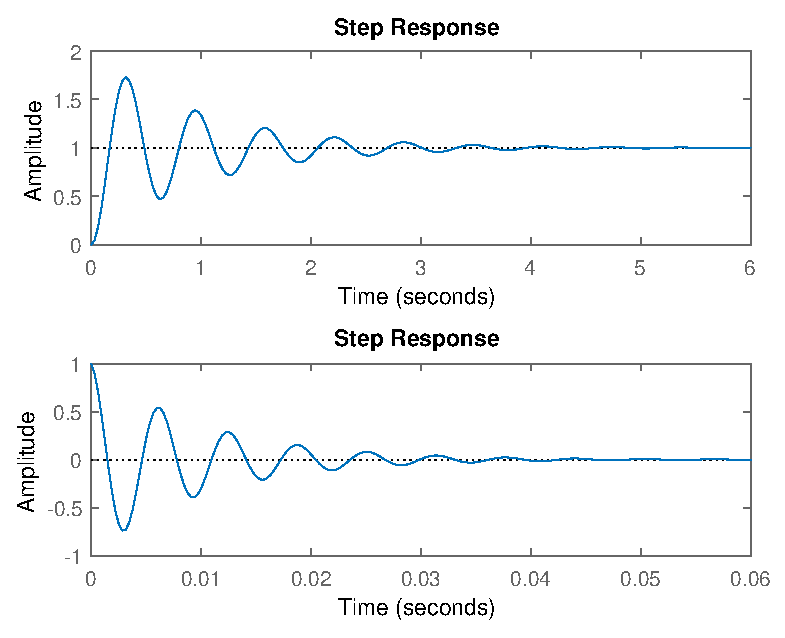
\includegraphics[width=0.6\textwidth]{Imagens/stepResponse.eps}
%	\caption[entrada]{Step response of both low-pass and high-pass modes.}
%	\label{fig:stepResponse}
%\end{figure}

\begin{figure}[!htb]
	\centering
	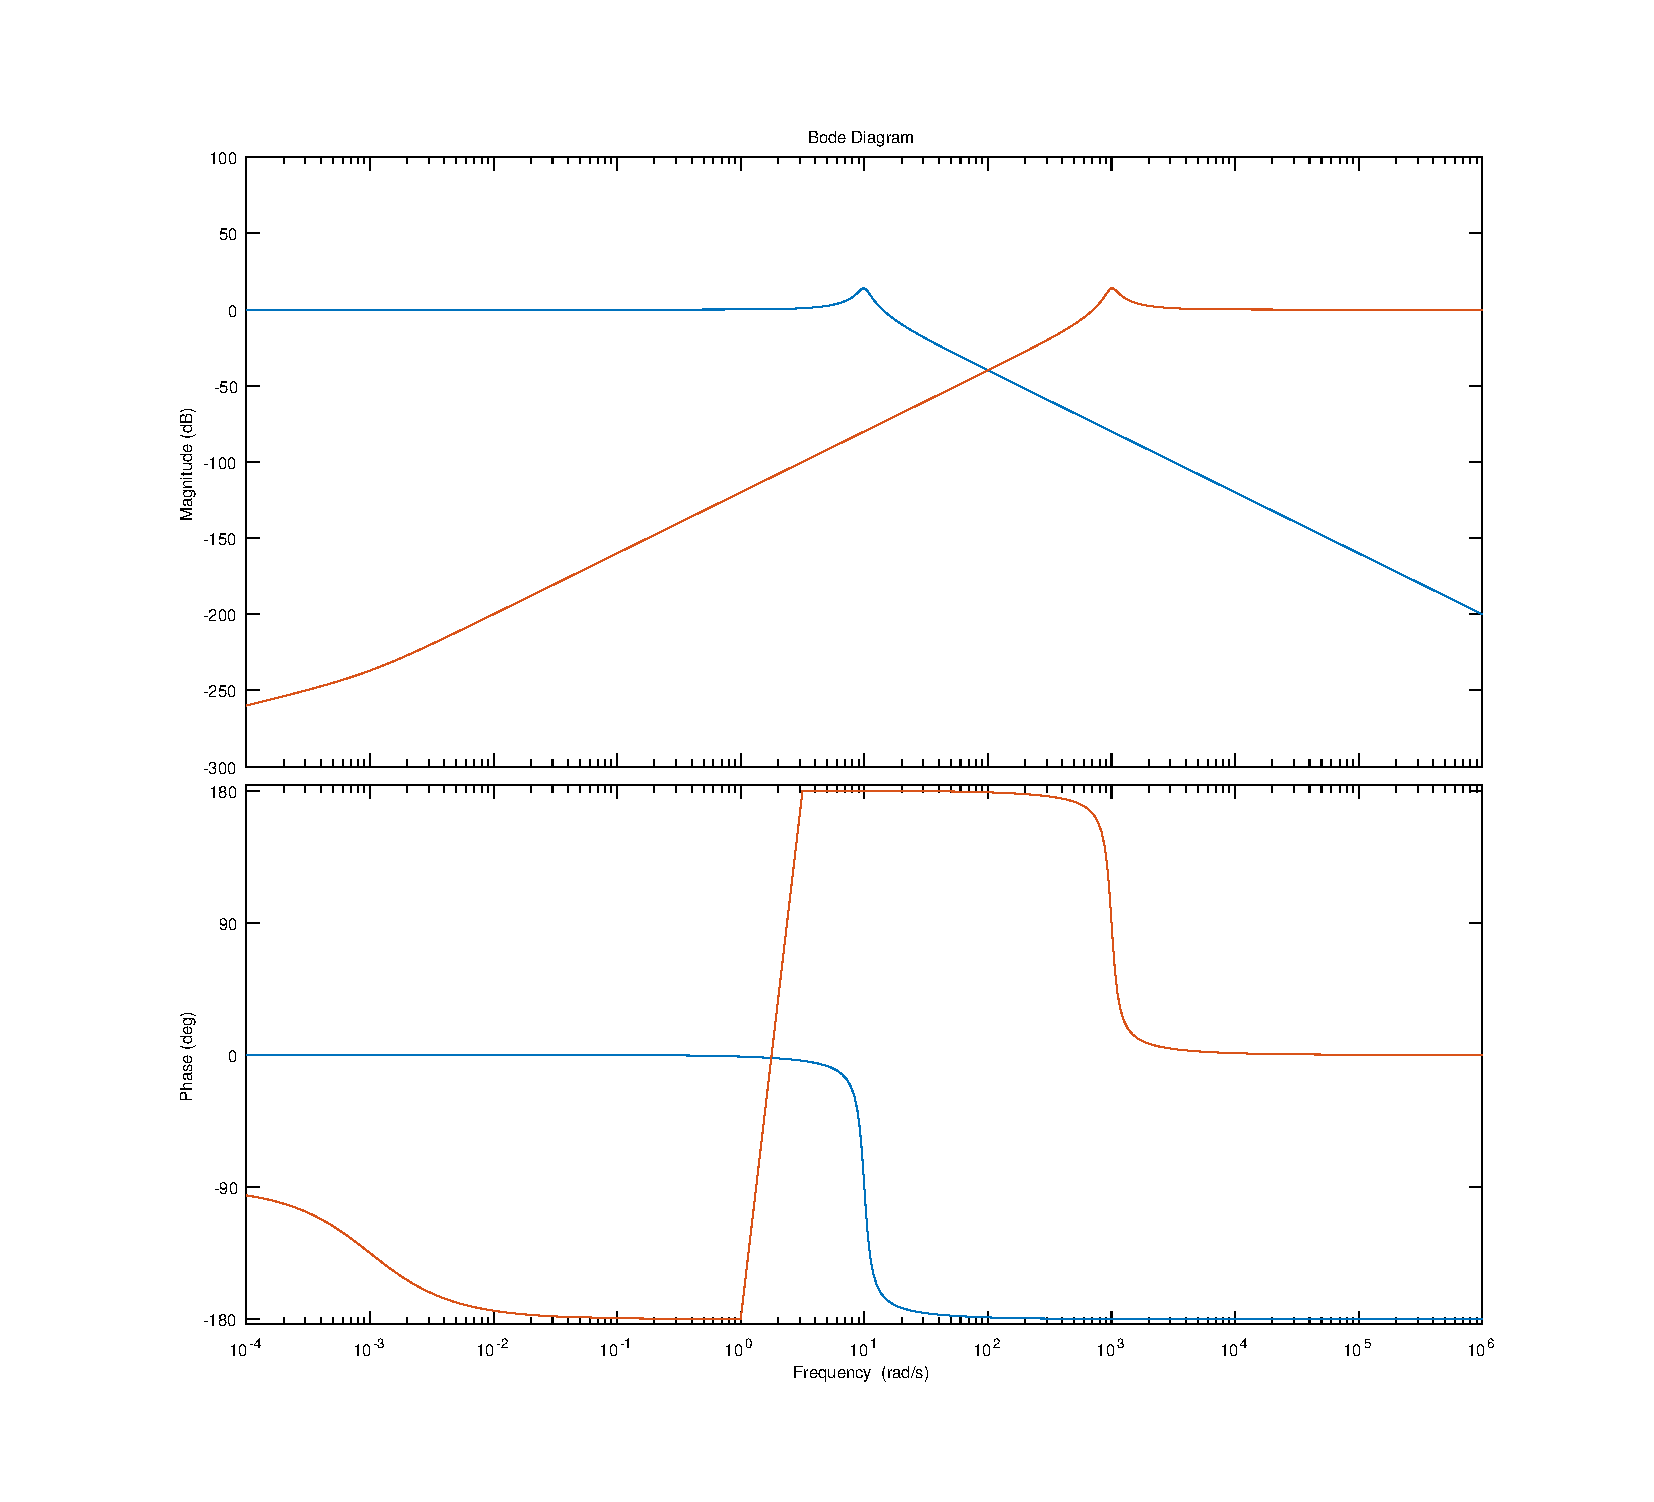
\includegraphics[width=0.8\textwidth]{Imagens/bode.eps}
	\caption[Bode diagram of both modes]{Bode diagram of both modes. Blue represent the low-pass system (\ref{eq:low-pass}) and red the high-pass system (\ref{eq:high-pass}).}
	\label{fig:bode}
\end{figure}

%\begin{figure}[!htb]
%	\centering
%	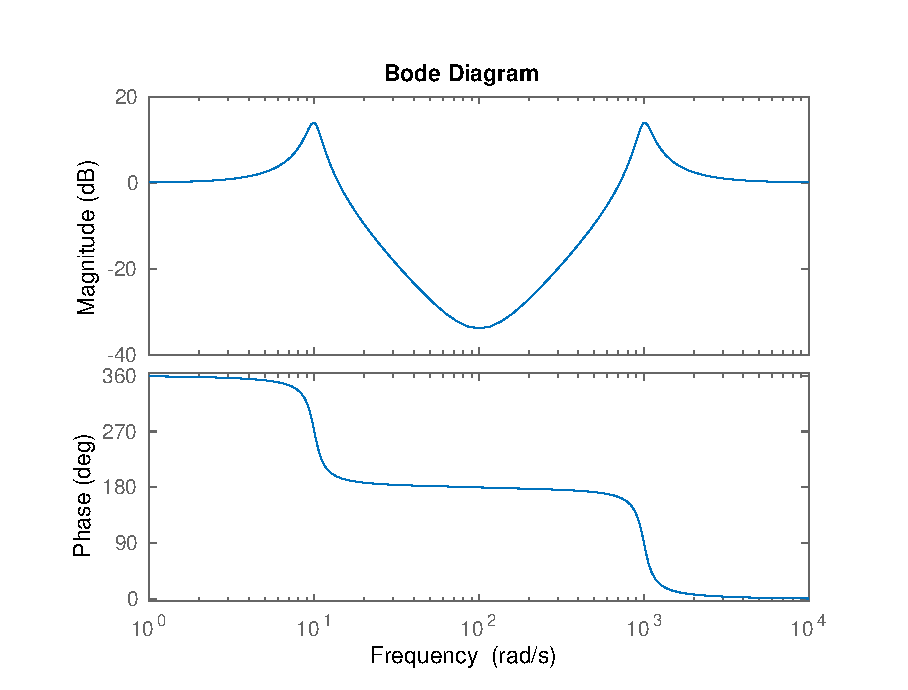
\includegraphics[width=0.6\textwidth]{Imagens/bodeS.eps}
%	\caption[entrada]{Bode diagram of the resulting fourth order system.}
%	\label{fig:bodeS}
%\end{figure}


The resulting fourth order system is described as a state space representation, in a modal canonical form given by:

\begin{align}
\dot{x}(t) & = Ax(t) + Bu(t) \label{eq:sys_beg}\\
y(t) & = Cx(t) + Du(t)
\end{align}


\noindent
where $x(t) \in \mathbb{R}^4$ is the state vector, $u(t) \in \mathbb{R}^1$ is the single input vector and $y(t) \in \mathbb{R}^1$ is the single output vector, and

\begin{align}
A & =\begin{bmatrix}
-100 & 994.99 & 0 & 0\\
-994.99 & -100 & 0 & 0\\
0 & 0 & -1 & 9.949\\
0 & 0 & -9.949 & -1
\end{bmatrix}, \label{eq:linear_A}\\
B & =\begin{bmatrix}
-24.6435 \\
-18.8943 \\
-4.1746 \\
-0.2675
\end{bmatrix}, \\
C & =\begin{bmatrix}
24.41 & -21.2522 & -0.1537 & 2.3977 \\
\end{bmatrix}, \\
D & =1. \label{eq:sys_end}
\end{align}

\noindent
Matrix $A$, given by (\ref{eq:linear_A}), indicates two subsystem dynamically decoupled. The upper diagonal block refers to the high-pass system (\ref{eq:high-pass}), whereas the lower diagonal block represents the low-pass system (\ref{eq:low-pass}).

%
%\begin{equation}\label{eq:sistemaLinear}
%\begin{split}
%Z_{de} & := (\partial Z/\partial \delta_e)/m = -61.655 \ m/s^2,\\
%Z_q & := (\partial Z/\partial q)/m = -5.132 \ m/s,\\
%Z_w & := (\partial Z/\partial W)/m = -3.1332 \ s^{-1},\\
%M_{de} & := (\partial M/\partial \delta_e)/I_y = -40.465 \ s^{-2},\\
%M_q & := (\partial M/\partial q)/I_y = -2.6864 \ s^{-1},\\
%M_w & := (\partial M/\partial W)/I_y = -0.04688 \ (s-m)^{-1},\\
%\tau & = 0.1 \ s \\
%U_o & = 306.42 \ m/s
%\end{split}
%\end{equation}

We simulate a pseudo-random binary sequence (PRBS) as input, with 200 samples, as shown in Figure~\ref{fig:prbs}. The PRBS signal is used as input to the low-pass and high-pass systems separately, considering two different time frames, of 2 and 20 seconds. The results of the four linear simulations are shown in Figure~\ref{fig:sys_results}. The 20 seconds simulation for the high-pass system achieve steady state values very quickly, with a dynamics hard to be observed. Thus, we choose the 2 seconds time frame to simulate the fourth order serialized systems, given by (\ref{eq:sys_beg})-(\ref{eq:sys_end}). The result of the linear simulation of the fourth order system is presented in Figure~\ref{fig:4ordersys2s}.


\begin{figure}[!htb]
	\centering
	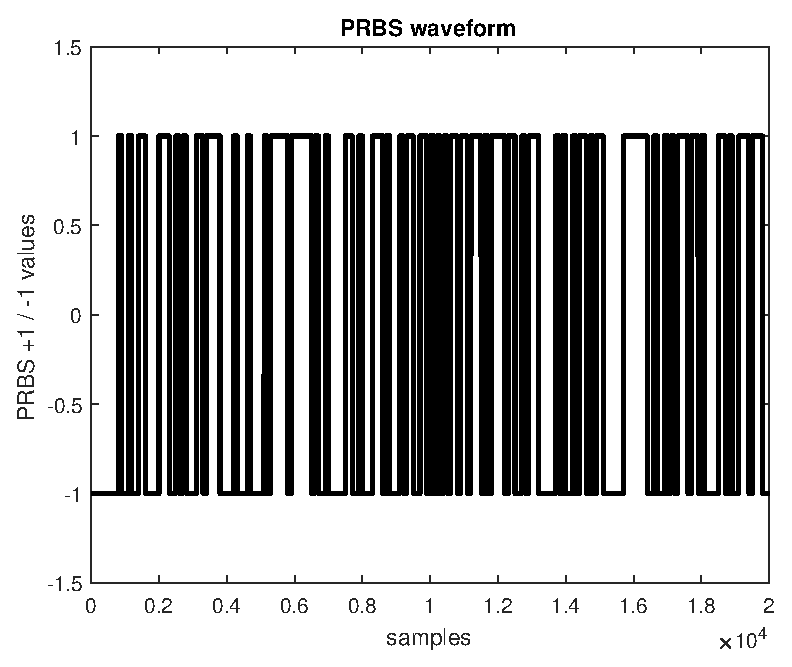
\includegraphics[width=0.75\textwidth]{Imagens/prbs.eps}
	\caption[PRBS samples used as input]{200 PRBS samples used as input to simulate system (\ref{eq:sys_beg})-(\ref{eq:sys_end})}
	\label{fig:prbs}
\end{figure}

\begin{figure}[!htb]
 	\centering
 	\subfigure[]{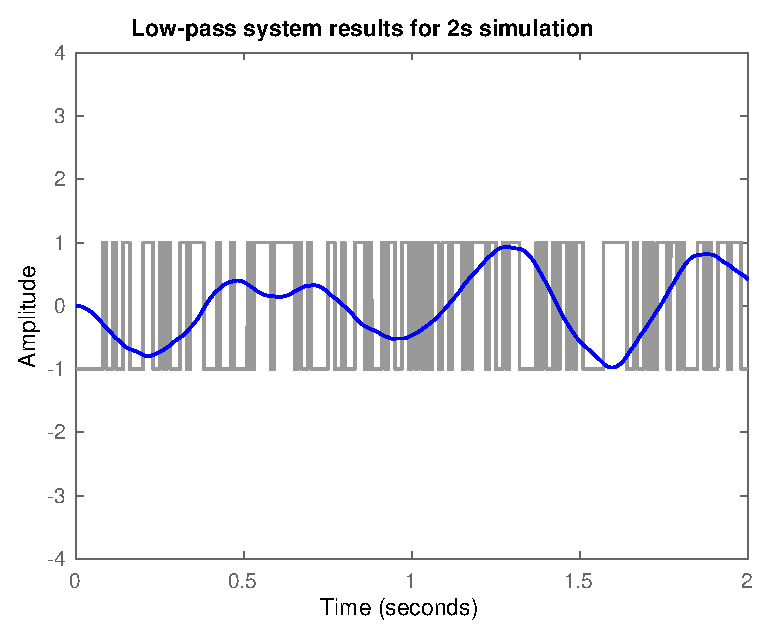
\includegraphics[width=0.49\textwidth]{Imagens/lp2s.eps}} 
 	\subfigure[]{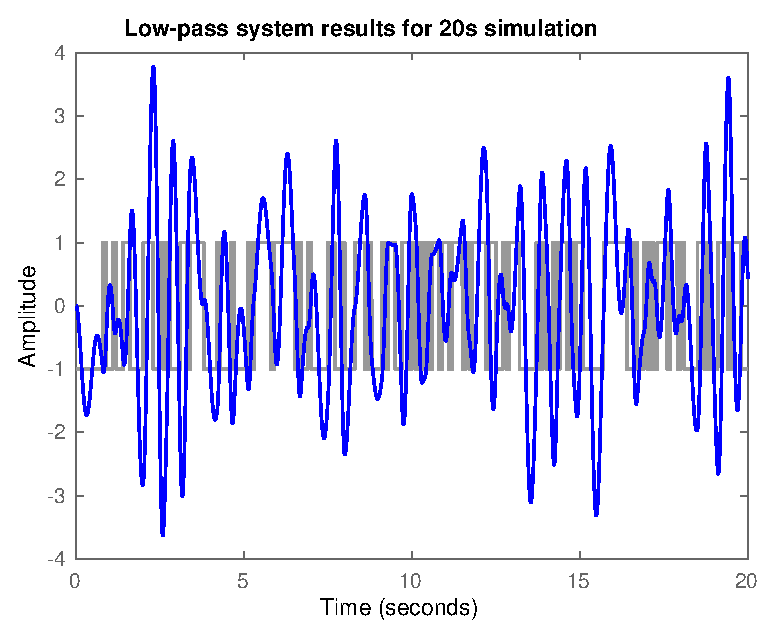
\includegraphics[width=0.49\textwidth]{Imagens/lp20s.eps}}  \\
 	\subfigure[]{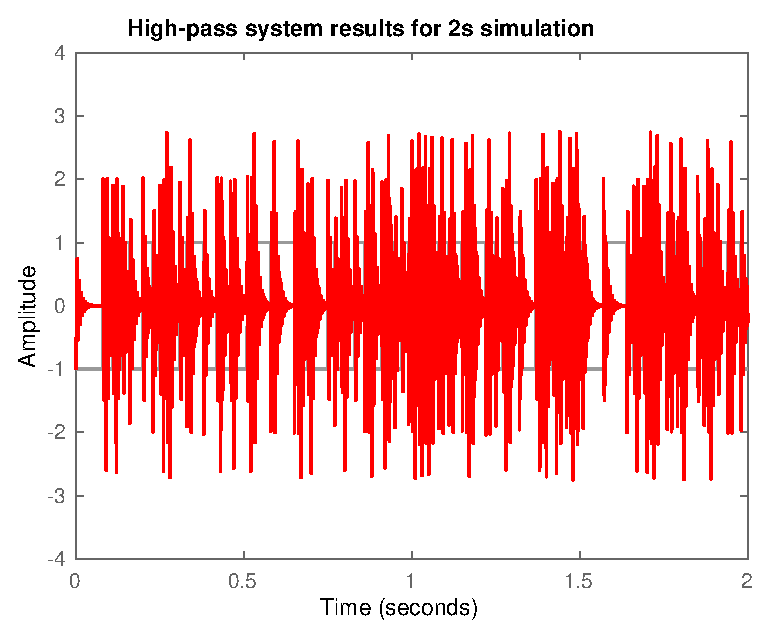
\includegraphics[width=0.49\textwidth]{Imagens/hp2s.eps}}
 	\subfigure[]{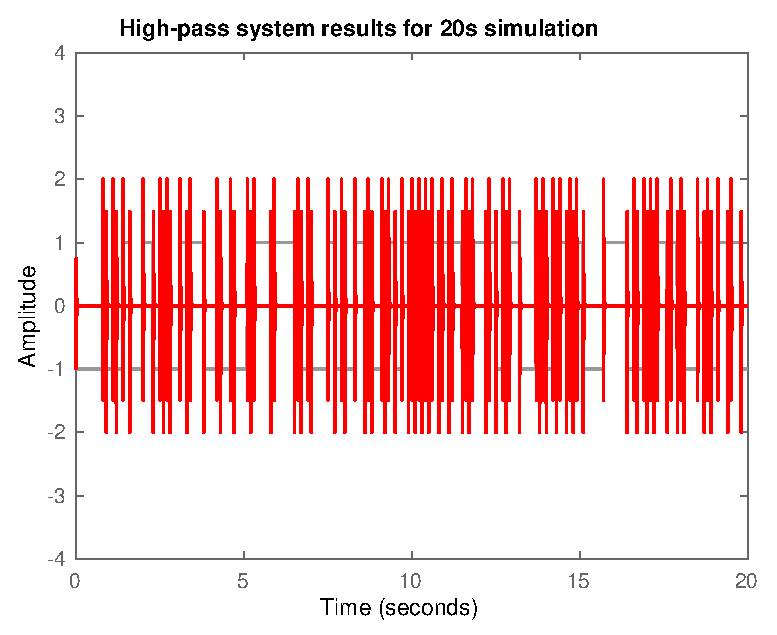
\includegraphics[width=0.49\textwidth]{Imagens/hp20s.eps}}
 	\caption[Linear simulation results for PRBS input in different time frames]{Linear simulation results of the low-pass and high-pass systems separately. Grey lines represent the PRBS input and colored lines the output. Graphs (a) and (b) with blue outputs represent the results of the low-pass system; and (c) and (d) with red outputs, the results of the high-pass system. Graphs on the left show a time frame of 2 seconds of simulations, whereas the ones on the right are the result of a 20 seconds time frame; considering the same 200 samples of PRBS for all four simulations.} 
 	\label{fig:sys_results}
 \end{figure}


\begin{figure}[!htb]
	\centering
	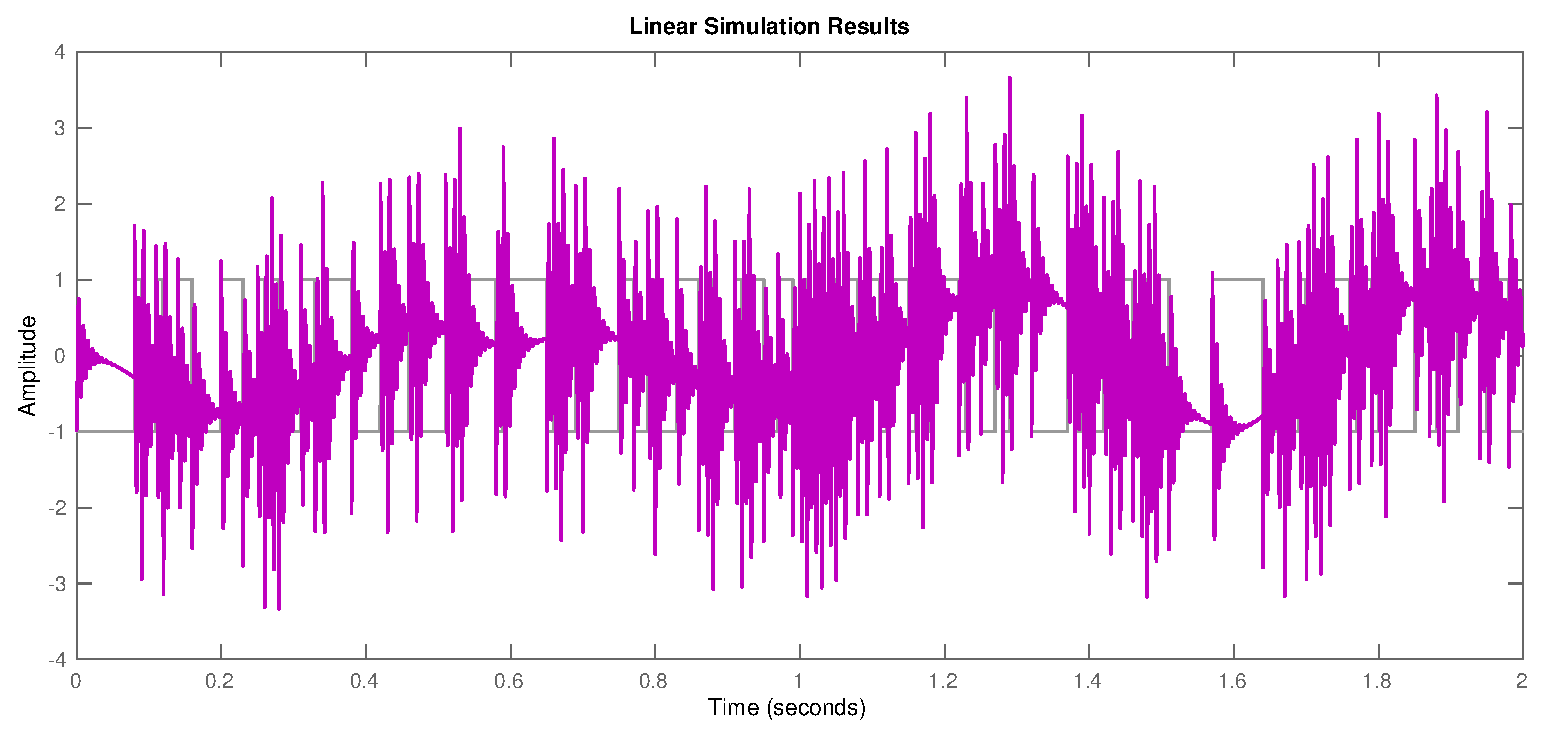
\includegraphics[width=0.8\textwidth]{Imagens/4ordersys2s.eps}
	\caption[Output of the fourth order system to the PRBS input signal]{Output of the fourth order system to the PRBS input signal over a 2 seconds time frame.}
	\label{fig:4ordersys2s}
\end{figure}

System discretization is performed using Matlab\texttrademark's built-in function \texttt{c2d} to produce a discrete-time state space representations according to

\begin{align}
x(t_{k+1}) &= A_{\textrm{d}}(t_k) x(t_k) + B_{\textrm{d}} u(t_k) + w(t_k), \\
y(t_k) &= B_{\textrm{d}}x(t)+D_{\textrm{d}}u(t) + v(t_k)
\end{align}

\noindent
where $t_{k+1} = t_k + h_k \in \mathbb{R}$ and $k \in \mathbb{N}$. $\rho(v(t_k)) = \mathcal{N} (0,R)$ and $\rho(w(t_k)) = \mathcal{N} (0,Q)$ are, respectively, the process and observation noise, with zero mean and covariance $R$ and $Q$. When time-stamp is not available, the observation vector is approximated by $\tilde{y}_i \approx y(t_k)$, where $i$ is the index of the next regular estimation time instant, multiple of $T$. When it is available, discretization is performed using variable time intervals.

\subsection{Linear System}

In this section we present one realization of the state estimation simulation for the system defined by (\ref{eq:sys_beg})-(\ref{eq:sys_end}), using the Kalman Filter described in Section~\ref{sec:kalman-filter} and the algorithms modifications explained in Section~\ref{sec:estimation_aperiodic}.  

Simulation parameters are set according to $\lambda = 500 \textrm{ Hz}$, $SNR_{\textrm{obs}} = 30 \textrm{ dB}$, and $SNR_{\textrm{pro}} = 30 \textrm{ dB}$, where subscript $\textrm{obs}$ and $\textrm{obs}$ refer to observation and process, respectively. Time step to simulate nominal system model is set as $\delta t_{\textrm{sim}} = 10^{-6} \textrm{ s}$ and the regular estimation time interval is given by $T = 2\times 10^{-3} \textrm{ s}$. Noise is generated using the \texttt{awgn} function from Matlab\texttrademark. For this realization, it resulted in a measurement noise variance of $R=9.596\times 10^{-4}$ and process noise variance of $Q=9.986\times 10^{-4}$. These exact values were used in the Kalman filter implementation and the estimation results for states $x_1$ and $x_4$ of the algorithms with and without timestamp, in comparison to the true state values are shown in Figures~\ref{fig:StatesWithAndWithoutTimeStamp}.

\begin{figure}[!htb]
	\centering
	\subfigure{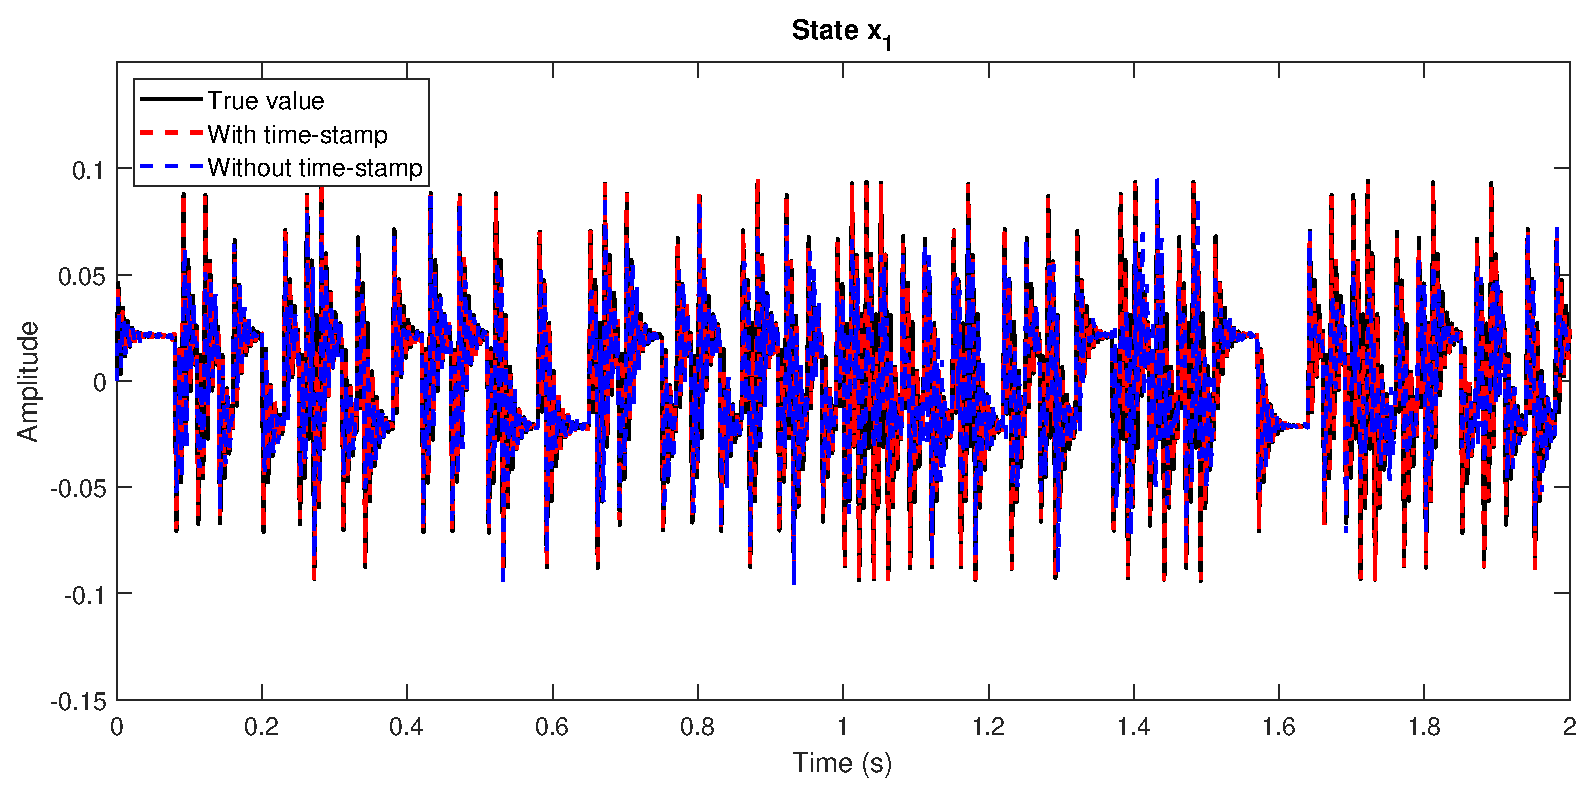
\includegraphics[width=0.8\textwidth]{Imagens/StatesWithTimeStamp.eps}} \\
	\subfigure{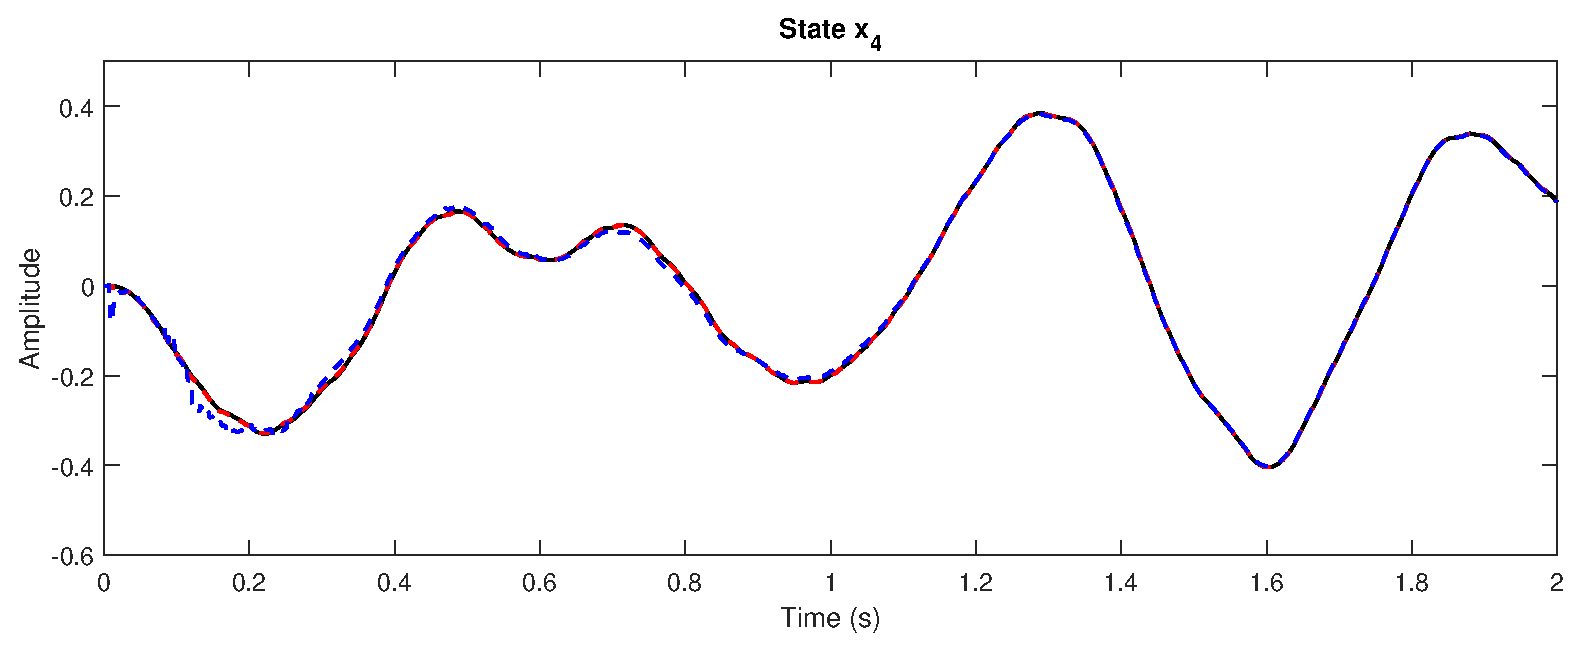
\includegraphics[width=0.8\textwidth]{Imagens/StatesWithoutTimeStamp.eps}}  
	\caption[Estimated and true states]{States $x_1$ and $x_4$ estimates with time-stamp (\textcolor{red}{- -}), without time-stamp (\textcolor{blue}{- -}) and true values (\textcolor{black}{---}).}
	\label{fig:StatesWithAndWithoutTimeStamp}
\end{figure}

For the high-pass subsystem state $x_1$, it is hard to note a significant difference in the estimation performance. However, for the low-pass system state $x_4$, the degradation is visible for the algorithm that does not acknowledge time instants $t_k$ information in the estimation process, represented by the dashed blue lines.


Figure~\ref{fig:LinearJevolution} presents a data window from 0 to 0.013 seconds of the accuracy index RMSE of state $x_2$, for the algorithms with and without time-stamp. As expected, when first observation arrives at $t_1$, RMSE results distance themselves, in favor of the algorithm that considers time-stamp. The RMSE difference increases the next measurement arrives at $t_2$. For the time period without observations, indexes of both algorithms evolve in a similar way. 
 	
\begin{figure}[!htb]
	\centering
	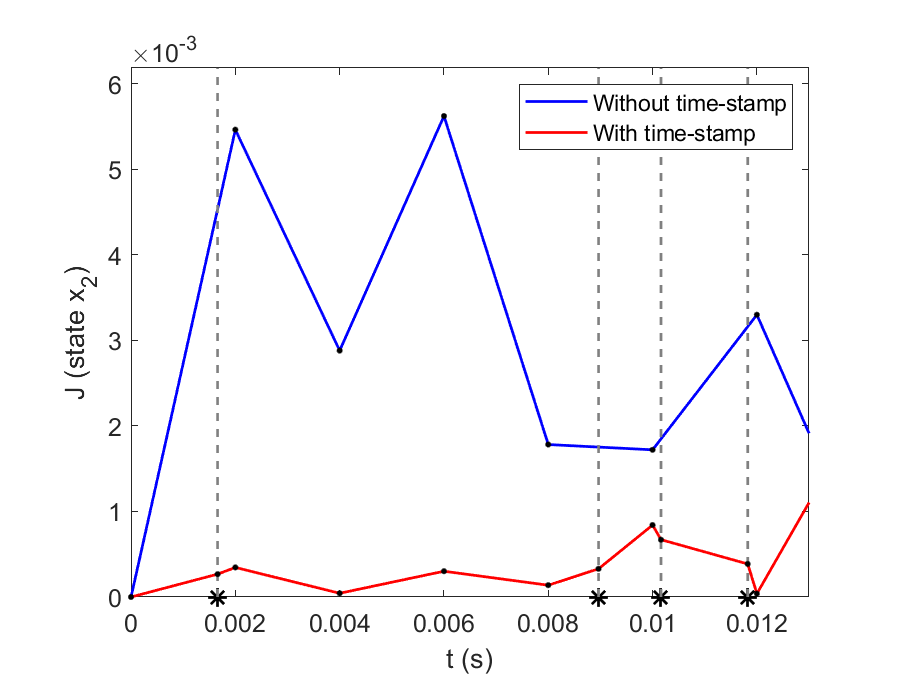
\includegraphics[width=0.8\textwidth]{Imagens/LinearJEvolution.eps}
	\caption[Performance index temporal cut for one realization]{Temporal cut from 0 to 0.013 seconds, for a realization of state $x_2$ RMSE for	 both estimators, with (\textcolor{red}{---}) and without (\textcolor{blue}{---}) time-stamp. Vertical dashed lines match the measurement sampling instants $t_k$. Black dots represent the estimation instants.}
	\label{fig:LinearJevolution}
\end{figure}

Finally, for this realization, we also present single-run consistency tests, using the indices NEES and NIS as defined in Section~\ref{sec:metrics} in Figure~\ref{fig:linearConsistency}. In each graph, the acceptance intervals are marked by horizontal lines. The upper plots (a) and (b) represent the NEES and NIS values, respectively, for the algorithm that considers time-stamp in the estimation process. We can see that the estimates are quite consistent, with the values inside the acceptance region most of the time. In fact, the null hypothesis rejection rate, that is the proportion of times the values were out of their acceptance region, was $4\%$ for NEES, and $5,5\%$ for NIS, very close the the $5\%$ expected. When time-stamp information was not available, consistency was heavily degraded, with rejection rates escalating to $61\%$ and $43\%$, respectively. Moreover, NEES and NIS values were so high in some occasions, that the acceptance region is hardly visible in the graphs. In practice, such a consistency degradation means that estimation covariances are highly underestimated.

 \begin{figure}[!htb]
	\centering
	\subfigure[]{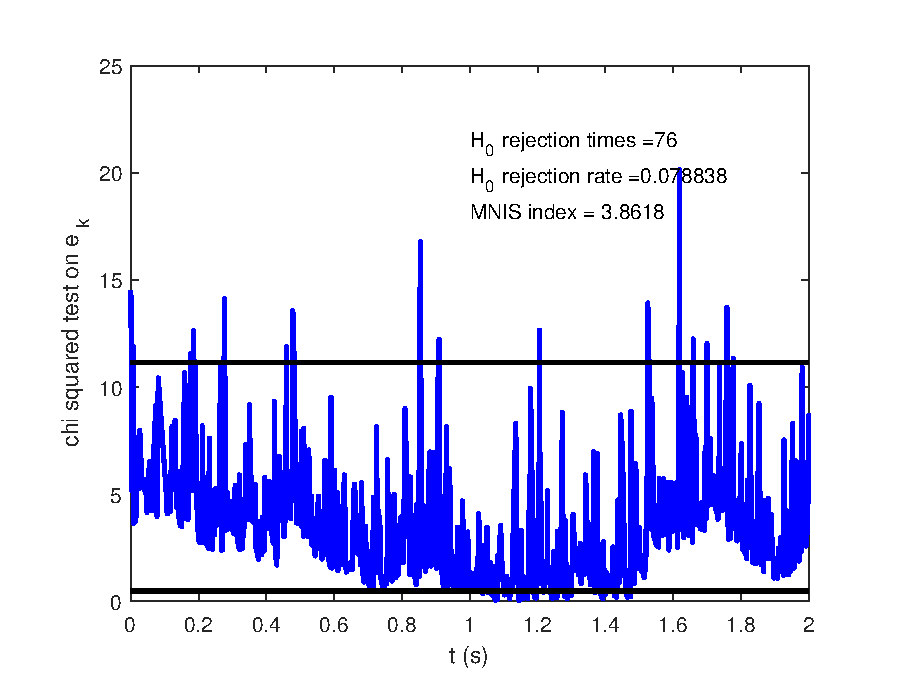
\includegraphics[width=0.49\textwidth]{Imagens/chi_e_with.eps}} 
	\subfigure[]{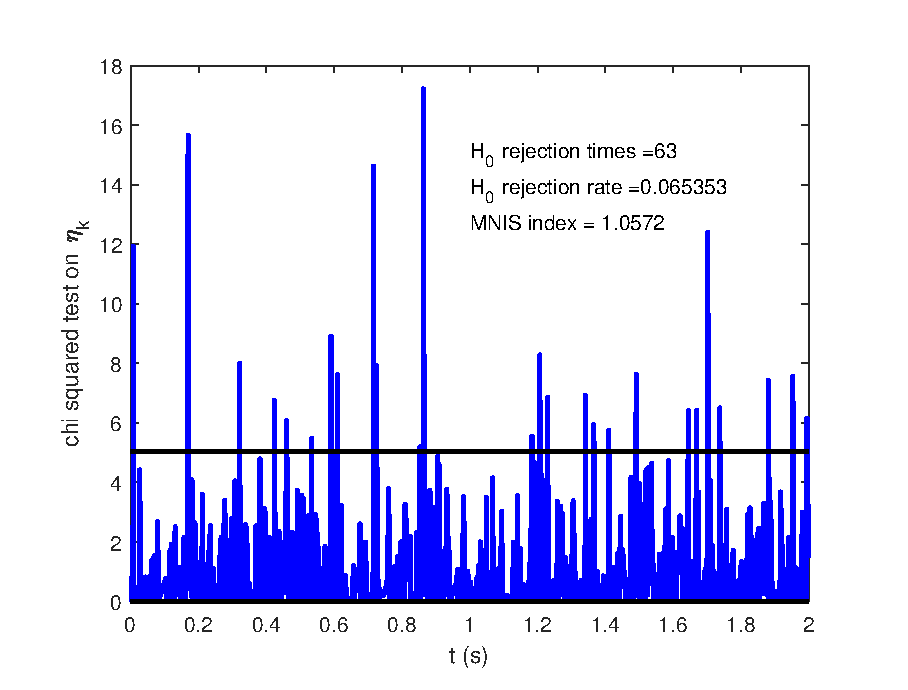
\includegraphics[width=0.49\textwidth]{Imagens/chi_eta_with.eps}}  \\
	\subfigure[]{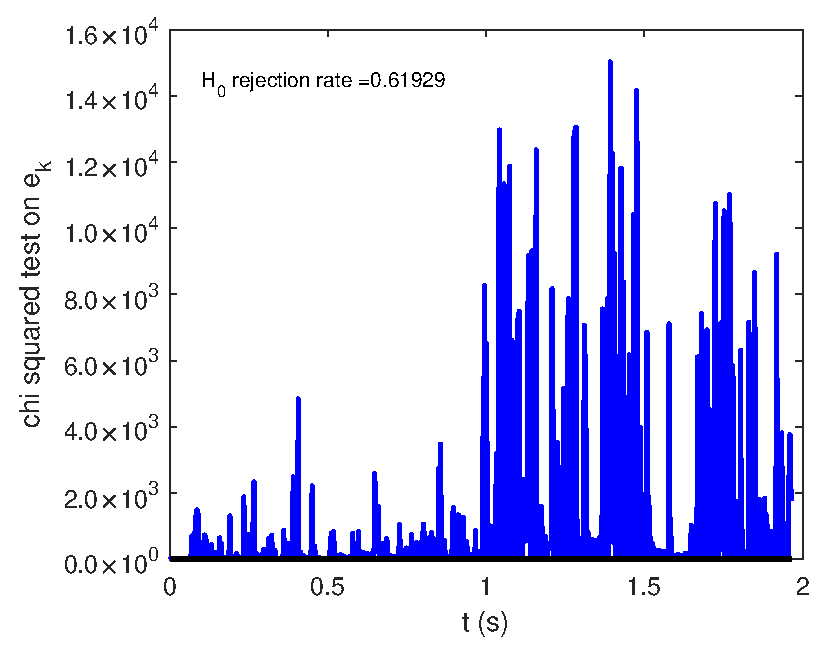
\includegraphics[width=0.49\textwidth]{Imagens/chi_e_without.eps}}
	\subfigure[]{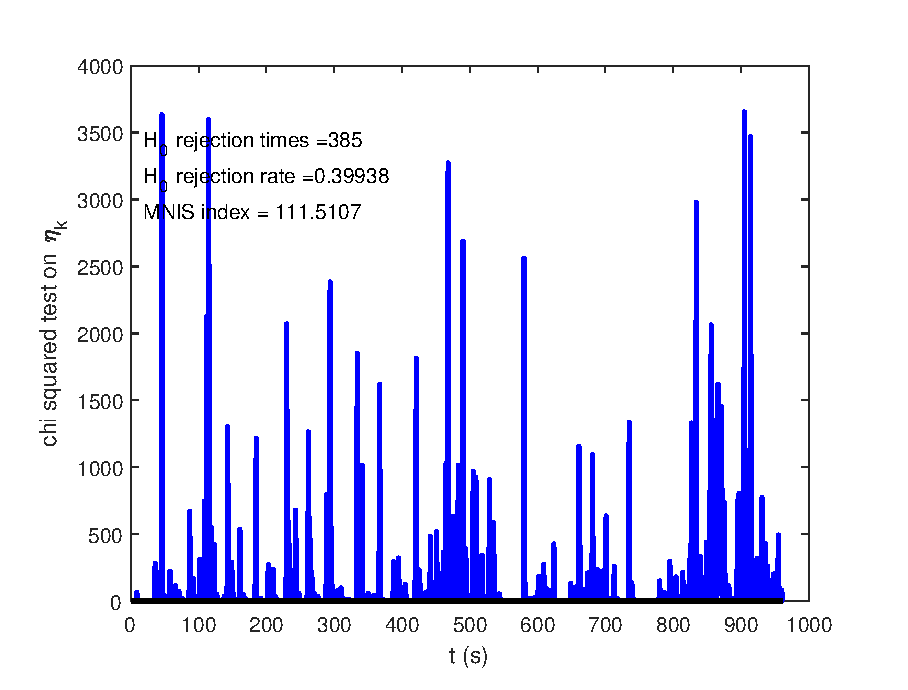
\includegraphics[width=0.49\textwidth]{Imagens/chi_eta_without.eps}}
	\caption[Consistency tests for linear system]{Consistency tests NEEs and NIS for the linear system state estimation with time-stamps (a) and (b); and without time-stamp (c) and (d). Horizontal lines define the acceptance region upper and lower limits, for a significance level $\alpha=0.05$. In each graph, the null hypothesis $H_0$ rejection rate is also presented.}
	\label{fig:linearConsistency}
\end{figure}

In the next sections we study the scenarios described in Section~\ref{sec:scenarios} for multiple runs. The simulation parameters are defined according to Table~\ref{tab:params_linear}
Only the results of one state per mode are shown, namely $x_1$ and $x_4$, for simplicity sake.. Figure~\ref{fig:linear_sim} encompasses results for all scenarios. Each column contains the performance metrics variation for each scenario. A 100-run Monte Carlo simulation was performed for each of them, and the mean and $95\%$ confidence intervals are presented for the algorithm with time-stamp in red and without time-stamp in blue.

\begin{table}[!ht]
	\centering
	\setlength{\tabcolsep}{12pt}	
	\caption[Linear system simulation parameters for SNR variation]{Linear system simulation parameters for SNR variation}
	\renewcommand{\arraystretch}{1.5}
	\small
	\begin{tabular}{c | c | c | c }
		\toprule
		Scenario & SNR (dB)	& $\lambda$ (Hz) & $\alpha$\\
		\midrule
		SNR variation & $[60,\ 50,\ 40,\ 20,\ 10]$	& $500$ & $1$ \\ 
		$\lambda$ variation & $30$		&  $[1000,\ 500,\ 200,\ 100]$ & $1$  \\ 
		$\alpha$ variation & $30$		&  $500$ & $[5,\ 3,\ 2,\ 1]$  \\ 
		\bottomrule
	\end{tabular}
	\label{tab:params_linear}
\end{table}

\subsection{Measurement Signal-to-Noise Ratio Variation}\label{sec:ruido-AC}

%For the first simulation scenario, we consider SNR variation for both the process and observation models jointly. Chosen parameters are presented in Table~\ref{tab:params_linear_snr} and results for the performance metrics are shown in column (a) of Figure~\ref{fig:linear_sim}.


%\begin{table}[!ht]
%	\centering
%	\setlength{\tabcolsep}{12pt}
%	\caption[Linear system simulation parameters for SNR variation]{Linear system simulation parameters for SNR variation}
%	\begin{tabular}{c | c | c }
%		\toprule
%		SNR (dB)	& $\lambda$ (Hz) & $\alpha$\\
%		\midrule
%		$[60,\ 50,\ 40,\ 20,\ 10]$	& $500$ & $1$ \\
%		\bottomrule
%	\end{tabular}
%	\label{tab:params_linear_snr}
%\end{table}

%Regular estimation time interval $T$ is maintained fixed at $T=0.002 \textrm{s}$  and $\alpha=1$, thus $\lambda=500 \textrm{Hz}$. For a 100-run simulation, the obtained results for accuracy and consistency are presented in Figure~\ref{fig:linearNoise} with the corresponding $95\%$ confidence intervals.


% \begin{figure}[!htb]
%	\centering
%	\subfigure[]{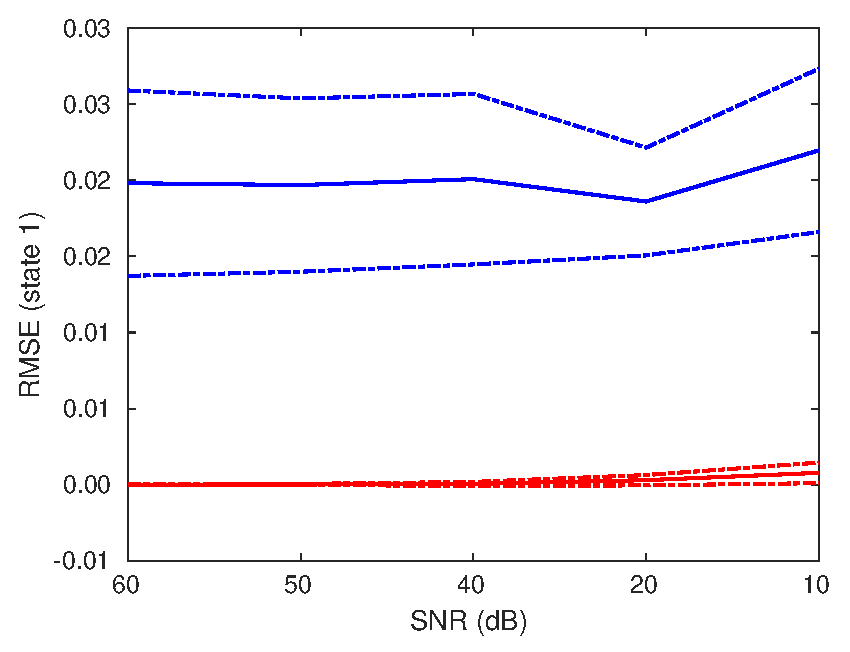
\includegraphics[width=0.49\textwidth]{Imagens/linearNoise_x1_rmse.eps}} 
%	\subfigure[]{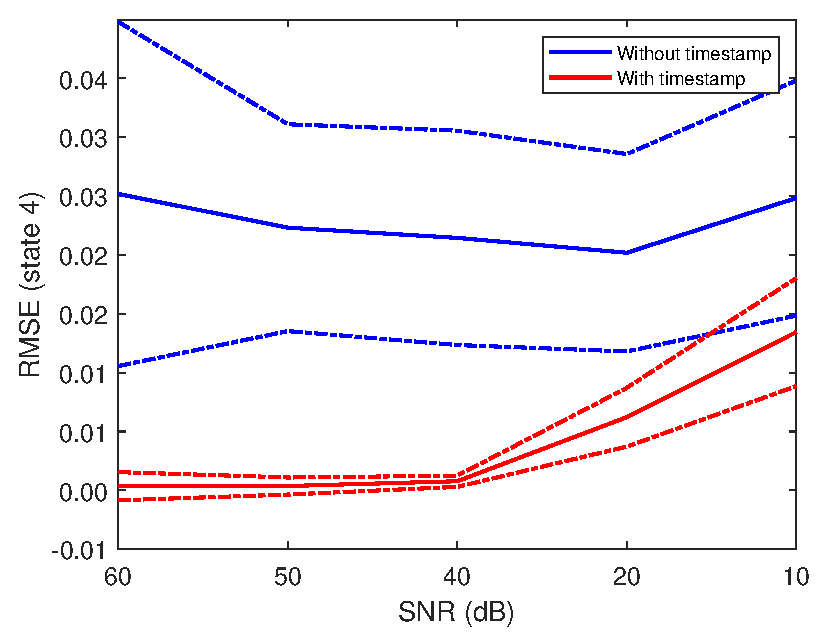
\includegraphics[width=0.49\textwidth]{Imagens/linearNoise_x4_rmse.eps}}  \\
%	\subfigure[]{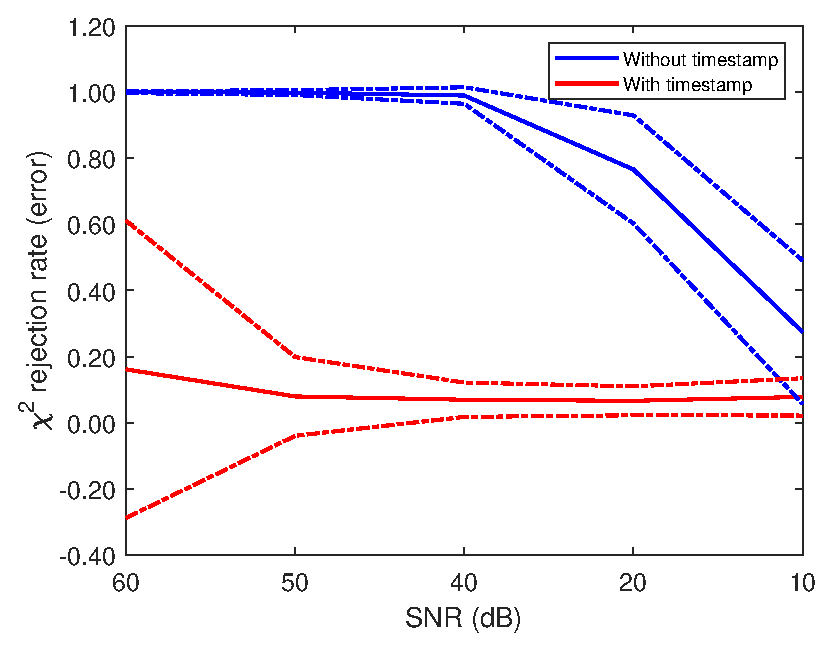
\includegraphics[width=0.49\textwidth]{Imagens/linearNoise_NEES.eps}}
%	\subfigure[]{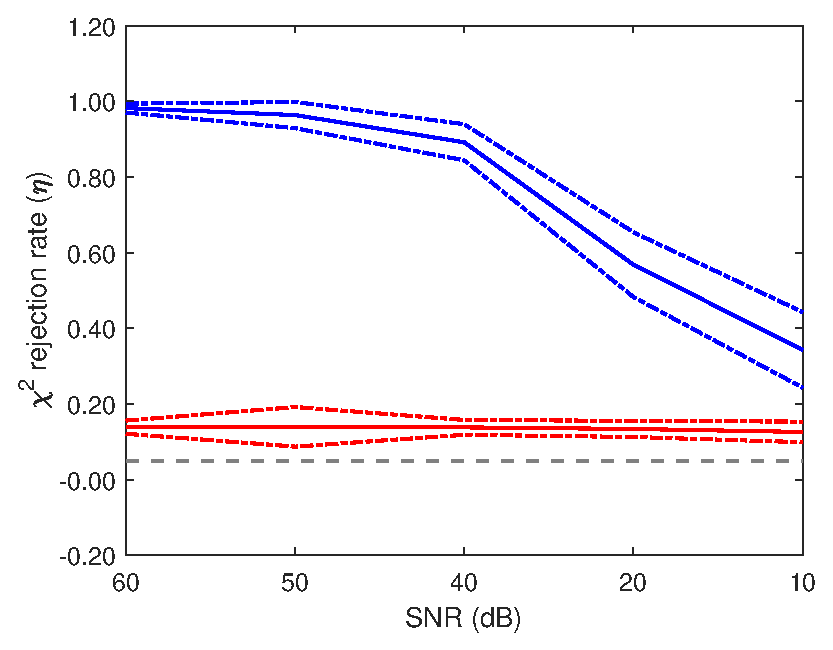
\includegraphics[width=0.49\textwidth]{Imagens/linearNoise_NIS.eps}}
%	\caption[Linear system estimation performance, as a function of input and observation SNR]{Linear system estimation performance indices with $95\%$ confidence intervals, as a function of input and observation SNR, for algorithms with (\textcolor{red}{---}) and without (\textcolor{blue}{---}) time-stamp. Accuracy values for states $x_1$ and $x_2$ are shown in (a) and (b), respectively. Consistency results are in (c) and (d) for NEES and NIS tests, respectively.}
%	\label{fig:linearNoise}
%\end{figure}

Results from the first column of Figure~\ref{fig:linear_sim} suggest that both agorithms with and without timestamp perform similarly for lower SNR in measurement and input data. When there is lower noise levels, there are apparent differences in estimation performance in favor of considering timestamp. 

There is a clear increasing trend for RMSE values of the algorithm considering timestamp, as expected, since state estimation with less noise in data should result in estimates closer to true values. As for consistency, considering time-stamp produces consistent estimates for all cases, with mean rates for NEES and NIS near the $5\%$ significance level.

The same behavior cannot be observed for the method without timestamp. In fact, RMSE results reduce for higher noise levels in data. Such behavior can be explained by the fact that for higher SNR, the additional noise tuned by assimilating data at incorrect time instants plays a more important role in the degradation of the estimates. When SNR decreases, the relevance of the additional noise caused by lack of timestamp is reduced. Estimates are more consistent and with less error in such scenarios.

\subsection{Average Sampling Rate Variation}\label{sec:lambda-AC}

%In the second simulation scenario for the linear system, we consider a variation of average sampling rate of observation $\lambda$, keeping other parameters fixed. Table~\ref{tab:params_linear_lambda} shows the used parameters and column (b) of Figure~\ref{fig:linear_sim}, the obtained results.

%
%\begin{table}[!ht]
%	\centering
%	\setlength{\tabcolsep}{12pt}
%	\caption[Linear system simulation parameters for $\lambda$ variation]{Linear system simulation parameters for $\lambda$ variation}
%	\begin{tabular}{c | c | c }
%		\toprule
%		SNR (dB)	& $\lambda$ (Hz) & $\alpha$ \\
%		\midrule
%		$30$		&  $[1000,\ 500,\ 200,\ 100]$ & $1$  \\
%		\bottomrule
%	\end{tabular}
%	\label{tab:params_linear_lambda}
%\end{table}

%
%$\lambda \ =\ 1000,\ 500,\ 20,\ \textrm{and } 10 \textrm{ Hz}$. Relation between $\lambda^{-1}$ and $T$ is kept constant $\alpha=1$. SNR levels for process and observation models are chosen to be $SNR_{\textrm{obs}} = SNR_{\textrm{pro}} = 30 \ \textrm{dB}$. Simulation was carried out 100 times and performance indices for accuracy and consistency are shown in Figure~\ref{fig:linearSamp} with corresponding $95\%$ confidence intervals. 
%
% \begin{figure}[!htb]
%	\centering
%	\subfigure[]{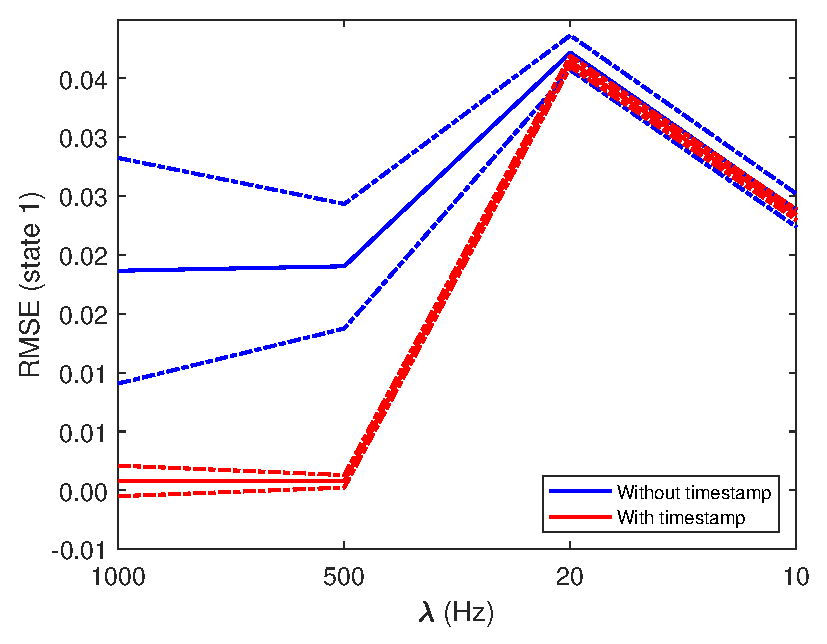
\includegraphics[width=0.49\textwidth]{Imagens/linearSamp_x1_rmse.eps}} 
%	\subfigure[]{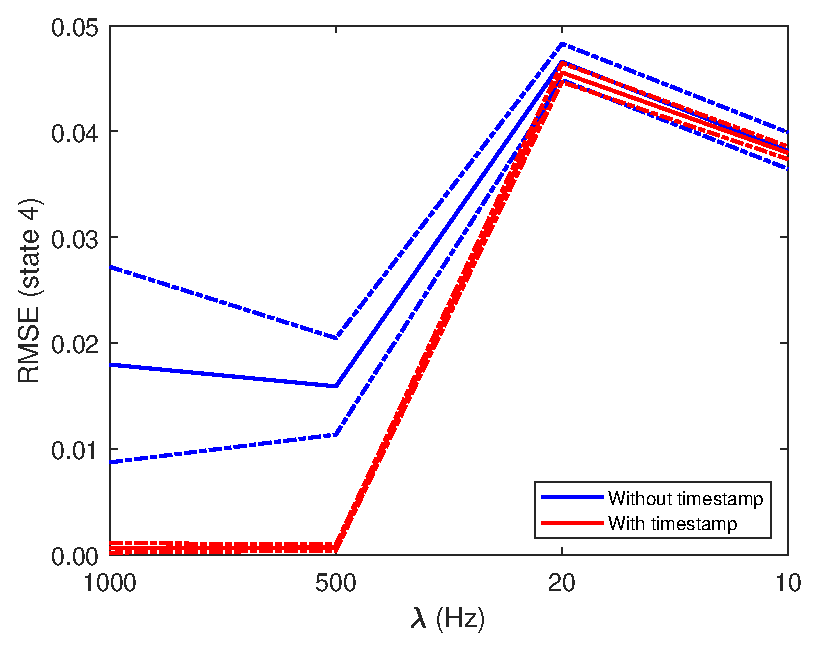
\includegraphics[width=0.49\textwidth]{Imagens/linearSamp_x4_rmse.eps}}  \\
%	\subfigure[]{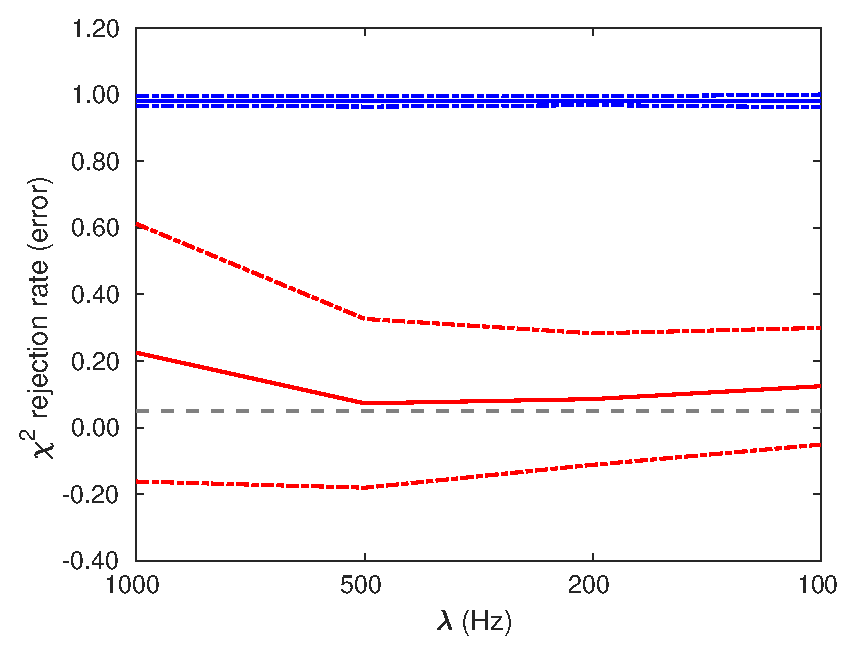
\includegraphics[width=0.49\textwidth]{Imagens/linearSamp_NEES.eps}}
%	\subfigure[]{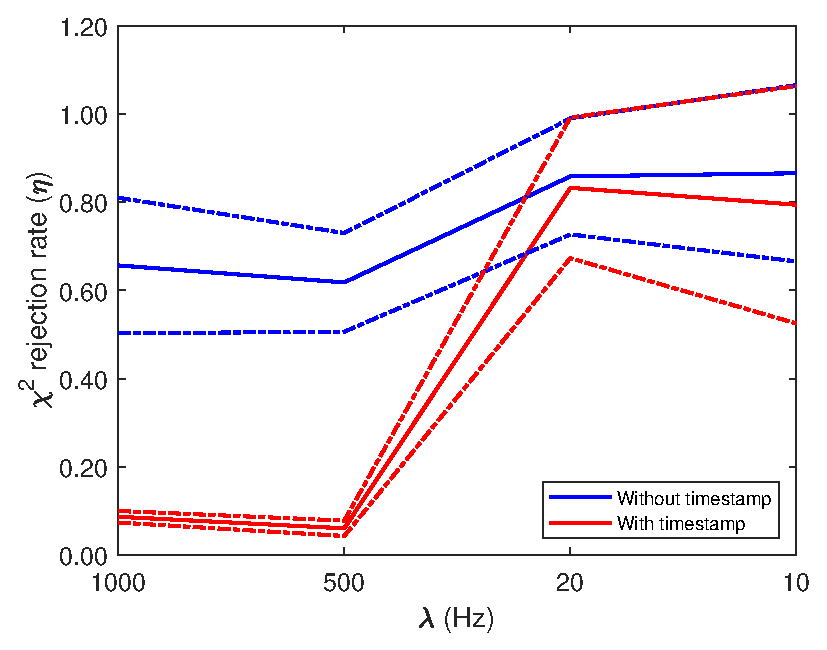
\includegraphics[width=0.49\textwidth]{Imagens/linearSamp_NIS.eps}}
%	\caption[Linear system estimation performance, as a function of input and observation SNR]{Linear system estimation performance indices with $95\%$ confidence intervals, as a function of average time interval $\lambda^{-1}$, for algorithms with (\textcolor{red}{---}) and without (\textcolor{blue}{---}) time-stamp. Accuracy values for states $x_1$ and $x_2$ are shown in (a) and (b), respectively. Consistency results are in (c) and (d) for NEES and NIS tests, respectively.}
%	\label{fig:linearSamp}
%\end{figure}

Variation of performance indices for $\lambda$ variation are shown in the second column of Figure~\ref{fig:linear_sim}. RMSE results for the high-pass system have such a high variability that it is hard to take any conclusions on the behavior. Mean RMSE for the algorithm with timestamp is systematically slower, however, and RMSE values are quite small, specially in comparison to results from the low-pass system. Graph (e), on the other hand, showing RMSE for low-pass system state $x_4$, suggest that for smaller average frequencies of the aperiodic sampled observations, not considering the exact time they were taken degrades accuracy greatly. That is expected, since the approximation errors of $\tilde{y}_i \approx y(t_k)$ are higher for more sparse average time intervals $1/\lambda$ and so is the additional noise introduced by data assimilation performed at incorrect time instants. We can also observe a small degradation for the algorithm with timestamp, which can be explained by discretization errors, increased for larger time steps.

Consistency performance results show that, for the parameter combinations simulated, not considering timestamp always underestimated errors, while the algorithm with timestamp achieved rejection rates consistently closer to $5\%$.  

\subsection{Regular and Average Irregular Time Interval Relation Variation}\label{sec:alpha-AC}

%The last linear system case study results, that is variation of $\alpha$, are shown in the third column of Figure~\ref{fig:linear_sim}. Used parameters are shown in Table~\ref{tab:params_linear_alpha} and results are presented in column (c) of Figure~\ref{fig:linear_sim}.


%\begin{table}[!ht]
%	\centering
%	\setlength{\tabcolsep}{12pt}
%	\caption[Linear system simulation parameters for $\alpha$ variation]{Linear system simulation parameters for $\alpha$ variation}
%	\begin{tabular}{c | c | c }
%		\toprule
%		SNR (dB)	& $\lambda$ (Hz) & $\alpha$ \\
%		\midrule
%		$30$		&  $500$ & $[5,\ 3,\ 2,\ 1]$  \\
%		\bottomrule
%	\end{tabular}
%	\label{tab:params_linear_alpha}
%\end{table}
%

% \begin{figure}[!htb]
%	\centering
%	\subfigure[]{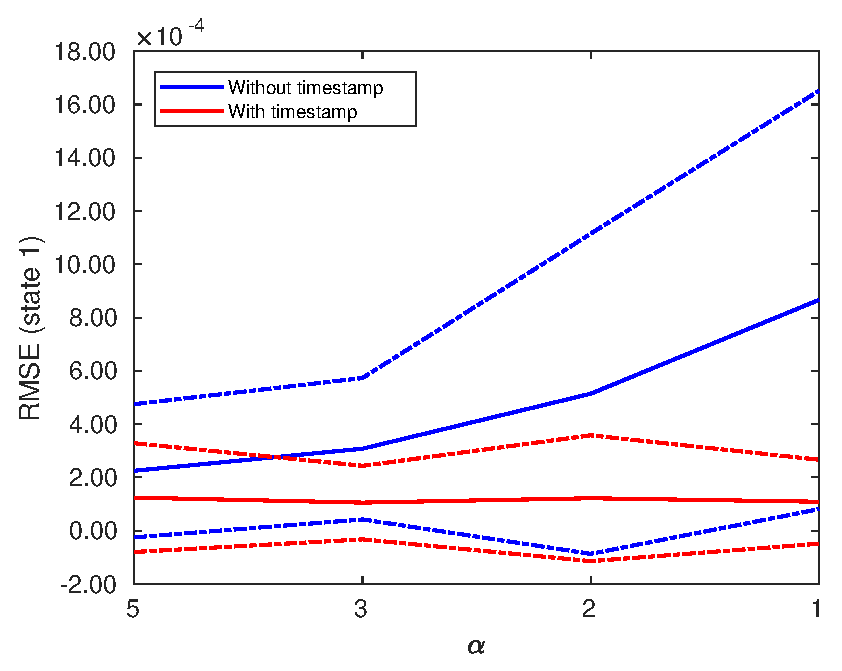
\includegraphics[width=0.49\textwidth]{Imagens/linearAlpha_x1_rmse.eps}} 
%	\subfigure[]{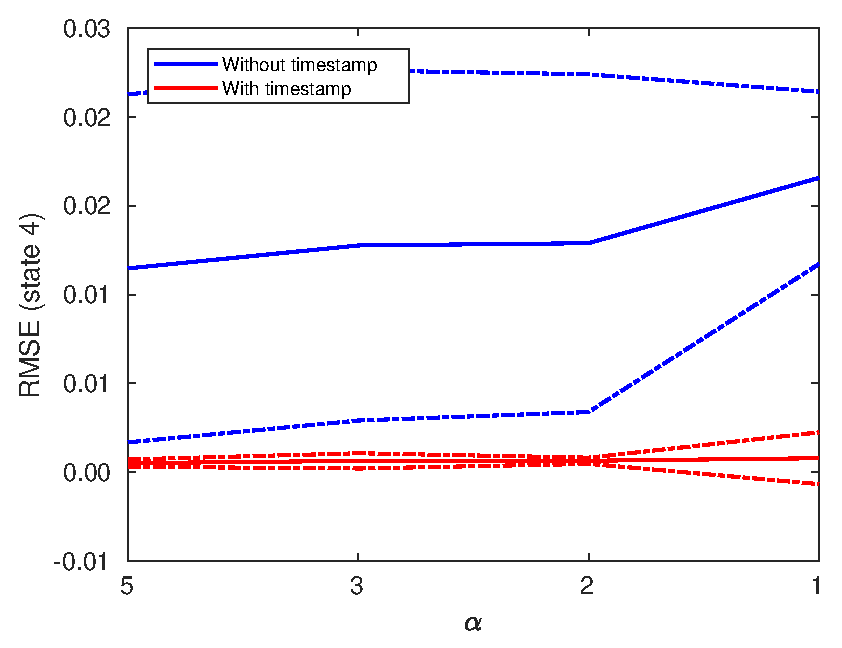
\includegraphics[width=0.49\textwidth]{Imagens/linearAlpha_x4_rmse.eps}}  \\
%	\subfigure[]{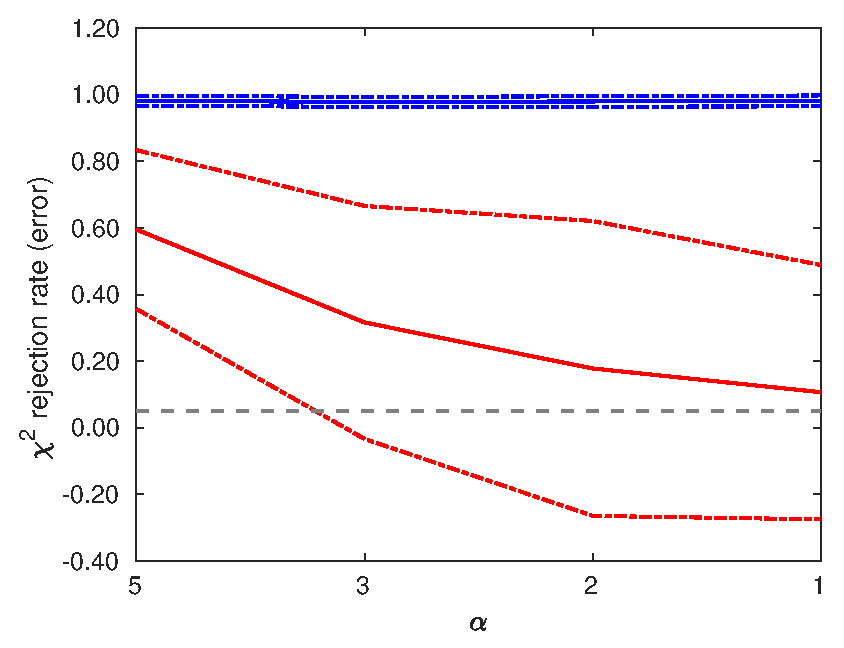
\includegraphics[width=0.49\textwidth]{Imagens/linearAlpha_NEES.eps}}
%	\subfigure[]{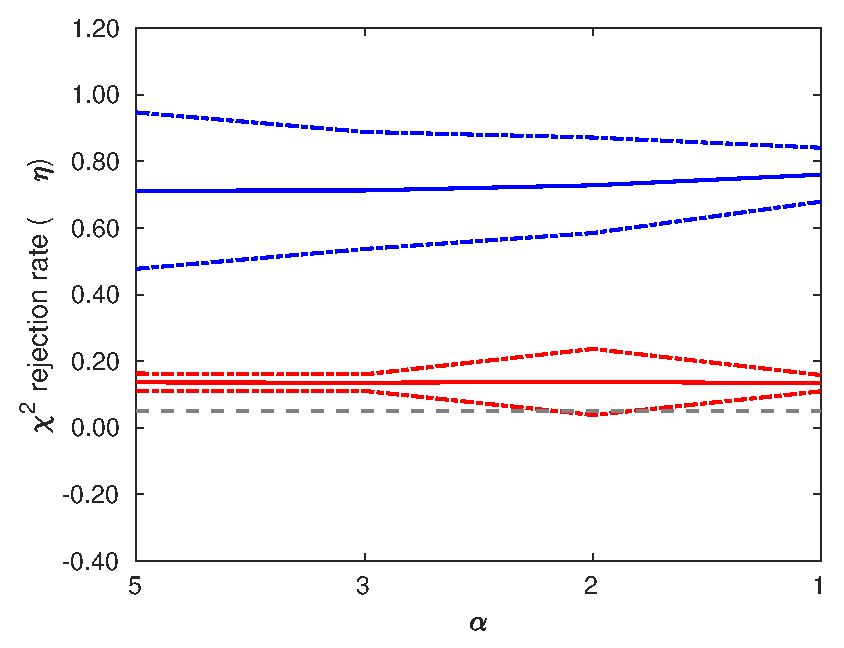
\includegraphics[width=0.49\textwidth]{Imagens/linearAlpha_NIS.eps}}
%	\caption[Linear system estimation performance, as a function of input and observation SNR]{Linear system estimation performance indices with $95\%$ confidence intervals, as a function of $\alpha$, for algorithms with (\textcolor{red}{---}) and without (\textcolor{blue}{---}) time-stamp. Accuracy values for states $x_1$ and $x_2$ are shown in (a) and (b), respectively. Consistency results are in (c) and (d) for NEES and NIS tests, respectively.}
%	\label{fig:linearAlpha}
%\end{figure}

Similarly to the variation of $\lambda$, changing values of $\alpha$ resulted in high variability in RMSE values for state $x_1$ with very small means. It is possible to observe an increasing trend of RMSE for the algorithm without timestamp, for smaller $\alpha$ values. The same trend is much more apparent in RMSE for low-pass system state $x_1$. On the other hand, state estimate errors for the algorithm with timestamp are small and apparently constant in all cases. It suggests that, the more sparse are the observation time intervals in comparison to the regular estimation time interval, that is the higher the $\alpha$, the more important it is assimilate data at the correct time instants $t_k$.

Again, consistency test results showed underestimated errors for the algorithm without timestamp systematically, whereas considering timestamp produced much more consistent estimates. 


 \begin{figure}[H]
	\centering
	\subfigure[SNR variation]{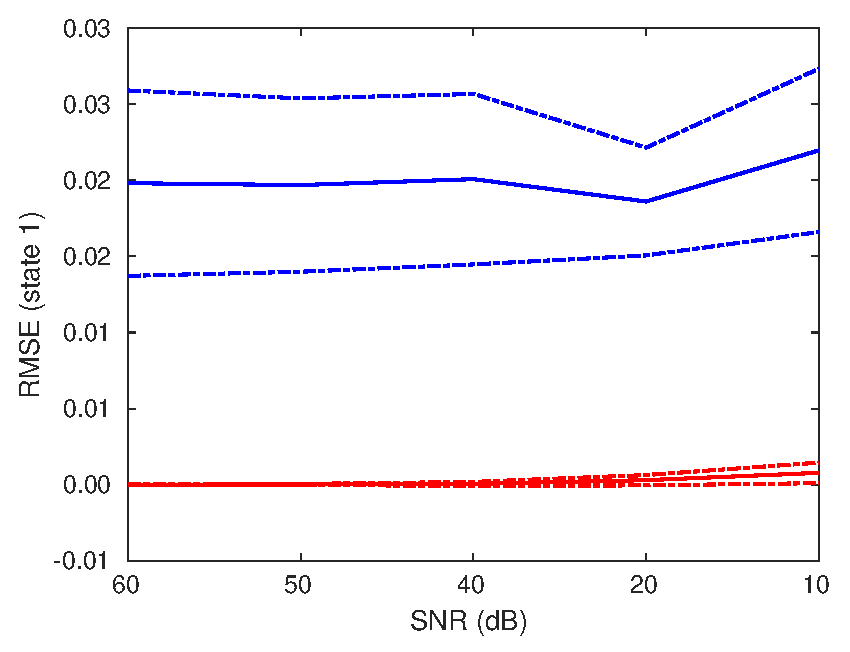
\includegraphics[width=0.32\textwidth]{Imagens/linearNoise_x1_rmse.eps}} 
	\subfigure[$\lambda$ variation]{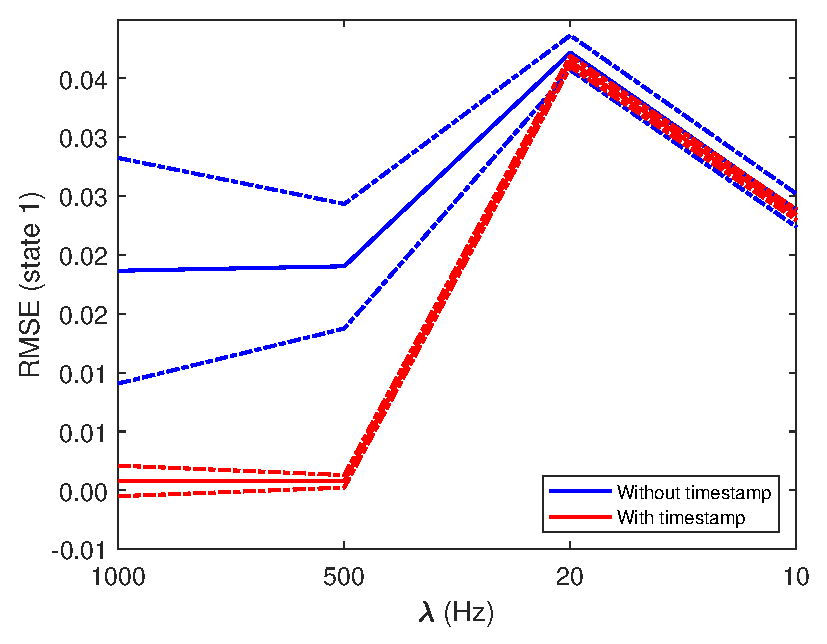
\includegraphics[width=0.32\textwidth]{Imagens/linearSamp_x1_rmse.eps}}  
	\subfigure[$\alpha$ variation]{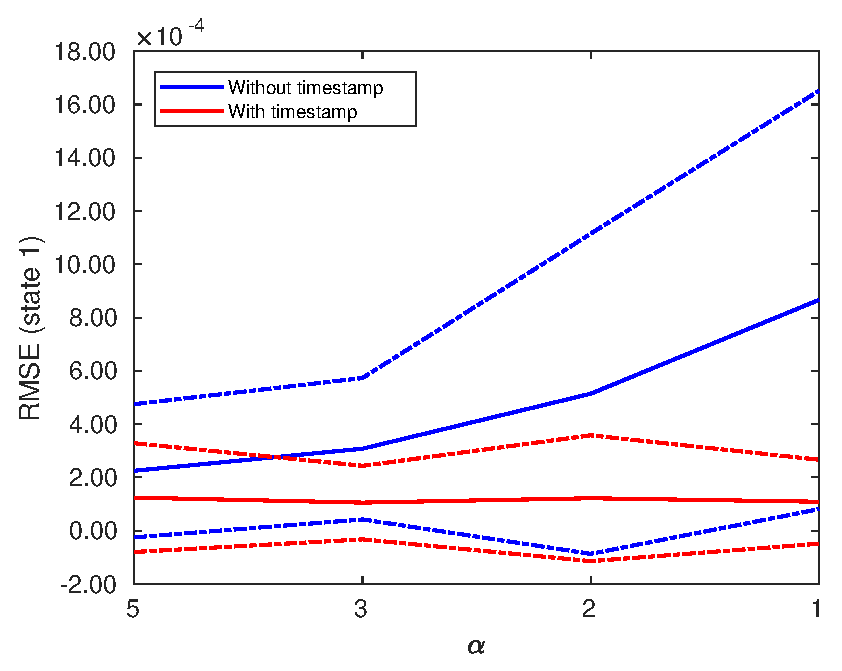
\includegraphics[width=0.32\textwidth]{Imagens/linearAlpha_x1_rmse.eps}} \\
	\subfigure[SNR variation]{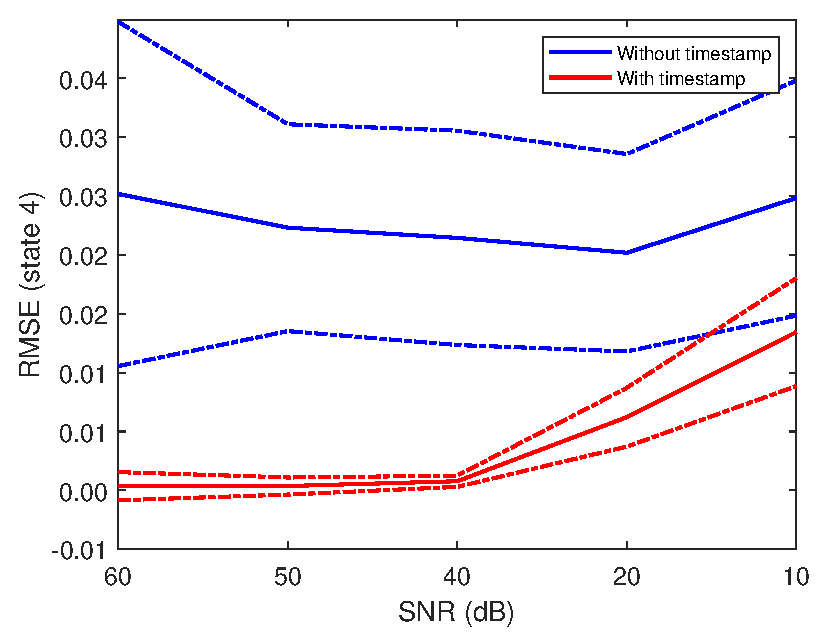
\includegraphics[width=0.32\textwidth]{Imagens/linearNoise_x4_rmse.eps}} 
	\subfigure[$\lambda$ variation]{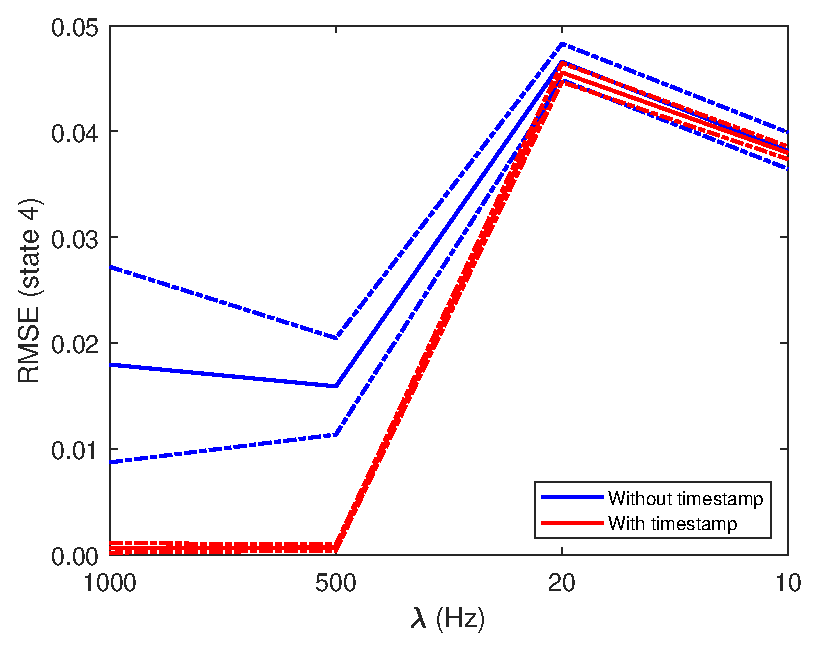
\includegraphics[width=0.32\textwidth]{Imagens/linearSamp_x4_rmse.eps}}  
	\subfigure[$\alpha$ variation]{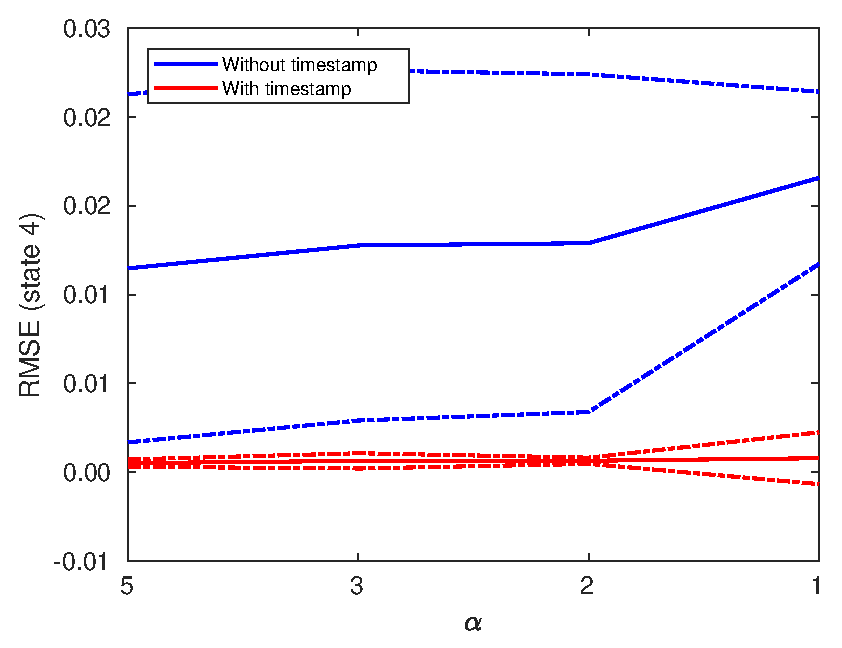
\includegraphics[width=0.32\textwidth]{Imagens/linearAlpha_x4_rmse.eps}} \\
	\subfigure[SNR variation]{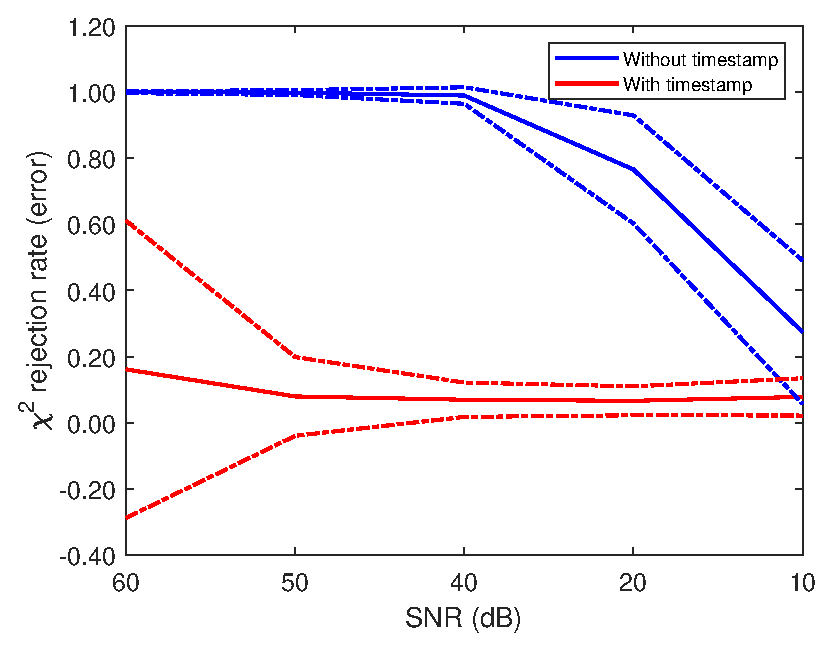
\includegraphics[width=0.32\textwidth]{Imagens/linearNoise_NEES.eps}} 
	\subfigure[$\lambda$ variation]{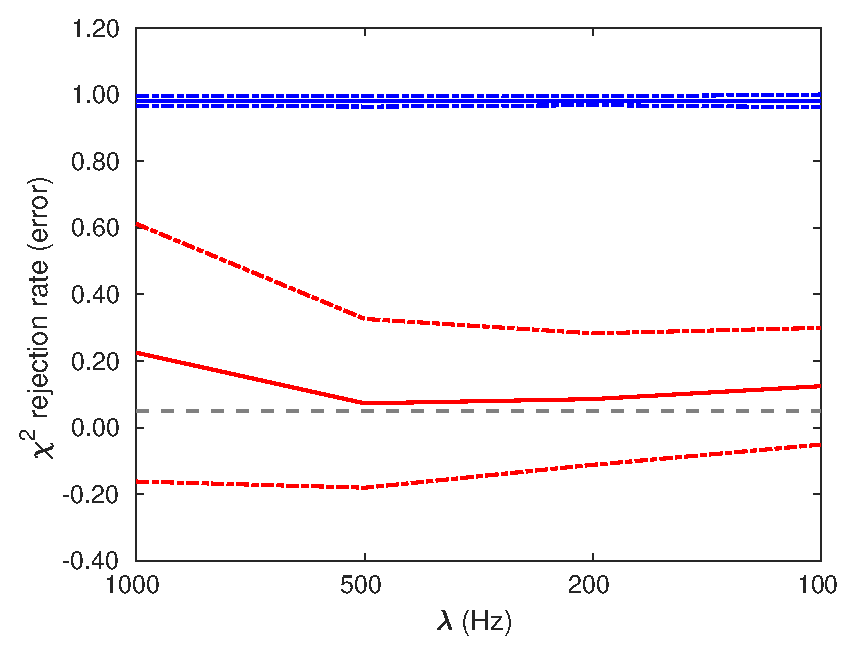
\includegraphics[width=0.32\textwidth]{Imagens/linearSamp_NEES.eps}}  
	\subfigure[$\alpha$ variation]{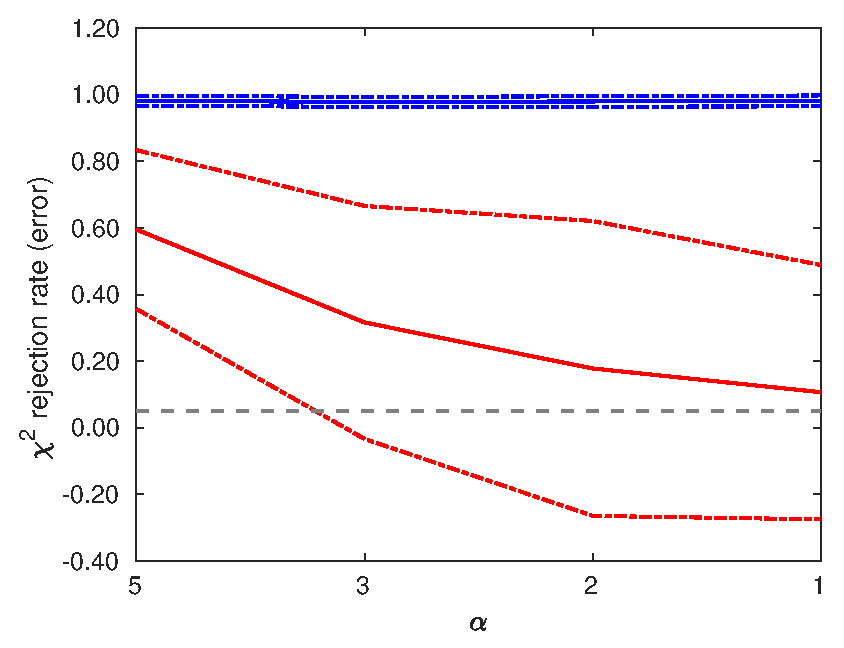
\includegraphics[width=0.32\textwidth]{Imagens/linearAlpha_NEES.eps}} \\
	\subfigure[SNR variation]{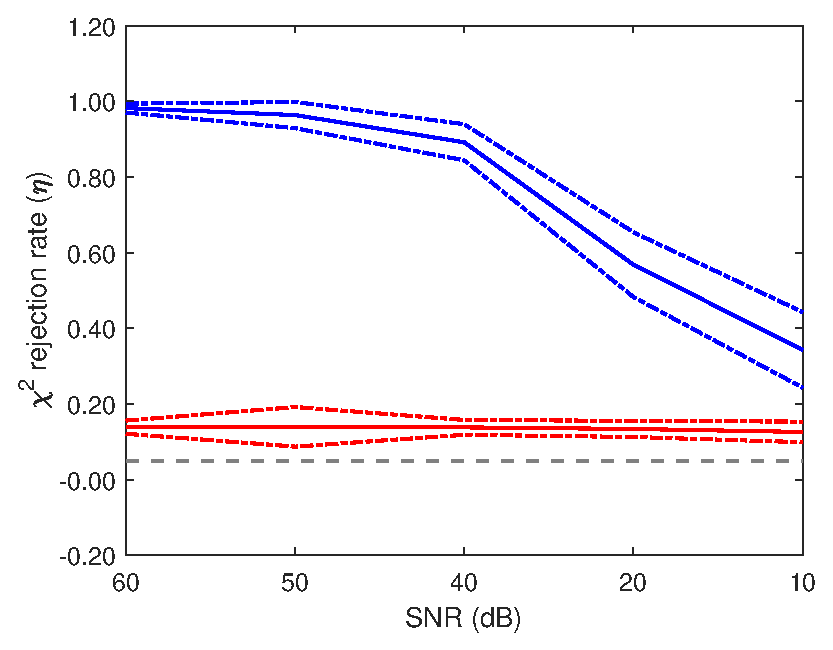
\includegraphics[width=0.32\textwidth]{Imagens/linearNoise_NIS.eps}} 
	\subfigure[$\lambda$ variation]{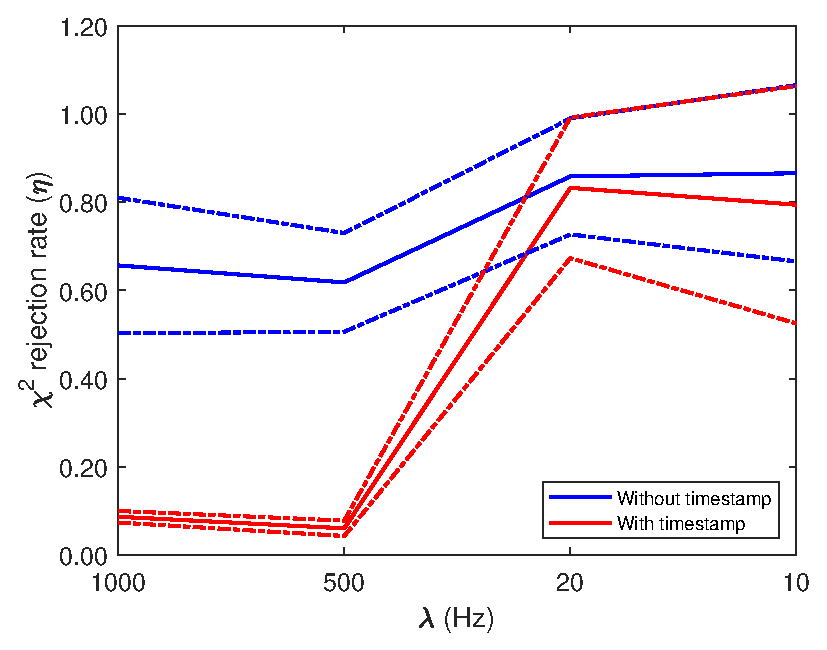
\includegraphics[width=0.32\textwidth]{Imagens/linearSamp_NIS.eps}}  
	\subfigure[$\alpha$ variation]{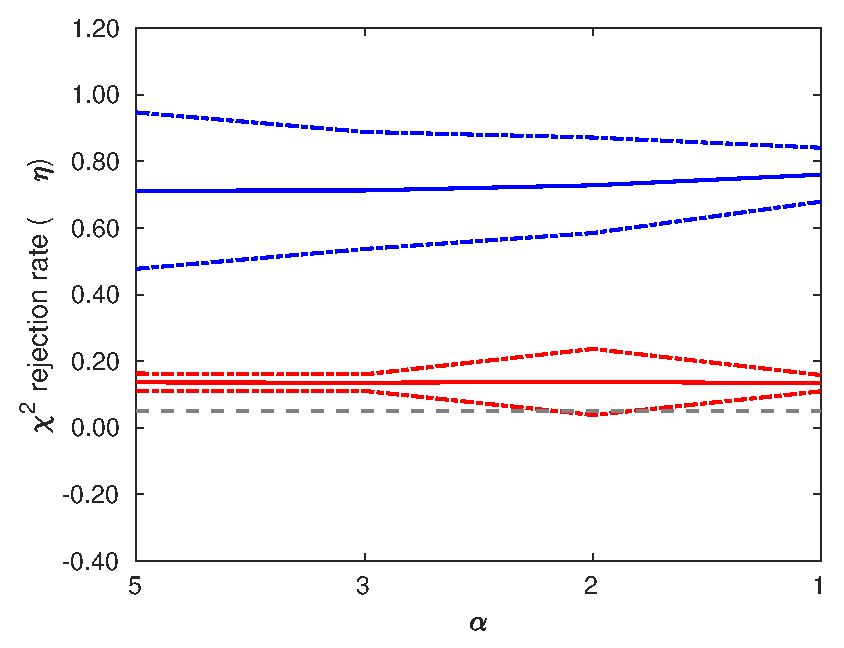
\includegraphics[width=0.32\textwidth]{Imagens/linearAlpha_NIS.eps}} \\
	\caption[Linear system estimation performance comparison]{Linear system estimation mean performance indices with $95\%$ confidence intervals, as a function of SNR (a,d,g,j), $\lambda$ (b,e,h,k) and $\alpha$ (c,f,i,l), considering (\textcolor{red}{---}) and not considering (\textcolor{blue}{---}) time-stamp. RMSE results are shown in the first ($x_1$) and second ($x_4$) rows. Consistency results are in third (NEES)) and fourth (NIS) rows. Horizontal gray dashed lines represent the $5\%$ significance level for the consistency tests.}
	\label{fig:linear_sim}
\end{figure}


%
%\subsection{Average Time Delay}\label{sec:dt-AC}
%
%\todo[inline,caption={Falta variar o atraso nas medi��es}]{Ainda ter� uma se��o com a varia��o do time-delay e seu impacto no desempenho}


\section{Nonlinear System: Unicycle Position}

We now consider a nonlinear system given by a nonholomonic moving unicycle robot, whose position in the $xy$-plane must be estimated. In many real target tracking problems such as this, measurements are available by unsynchronized cameras through an internet network, for instance. In other applications multiple GPS sensors might be used in a centralized architecture without data alignment or association. These configurations are susceptible to sampling irregularities, which motivates our choice.

\subsection{System Description}

Consider a nonholomonic moving robot, with the cinematic process model given by

\setlength{\abovedisplayskip}{0.5pt}

\begin{equation}\label{eq:sistema}
\begin{split}
\dot{p}_\textrm{x} & = v\cos (\theta),\\
\dot{p}_\textrm{y} & = v\sin (\theta),\\
\dot{\theta}  & = u_1(t),\\
\dot{v} & = u_2(t),
\end{split}
\end{equation}

\noindent
where $p_\textrm{x}$ and $p_\textrm{y}$ are the position coordinates, $\theta$ the angular orientation, $v$ the linear velocity and inputs $u_1$ and $u_2$ are the angular velocity $\omega$ and the linear acceleration $a$, respectively. Figure~\ref{fig:robot} shows a schematic of the robot and its states,

\begin{figure}[!htb]
	\centering
	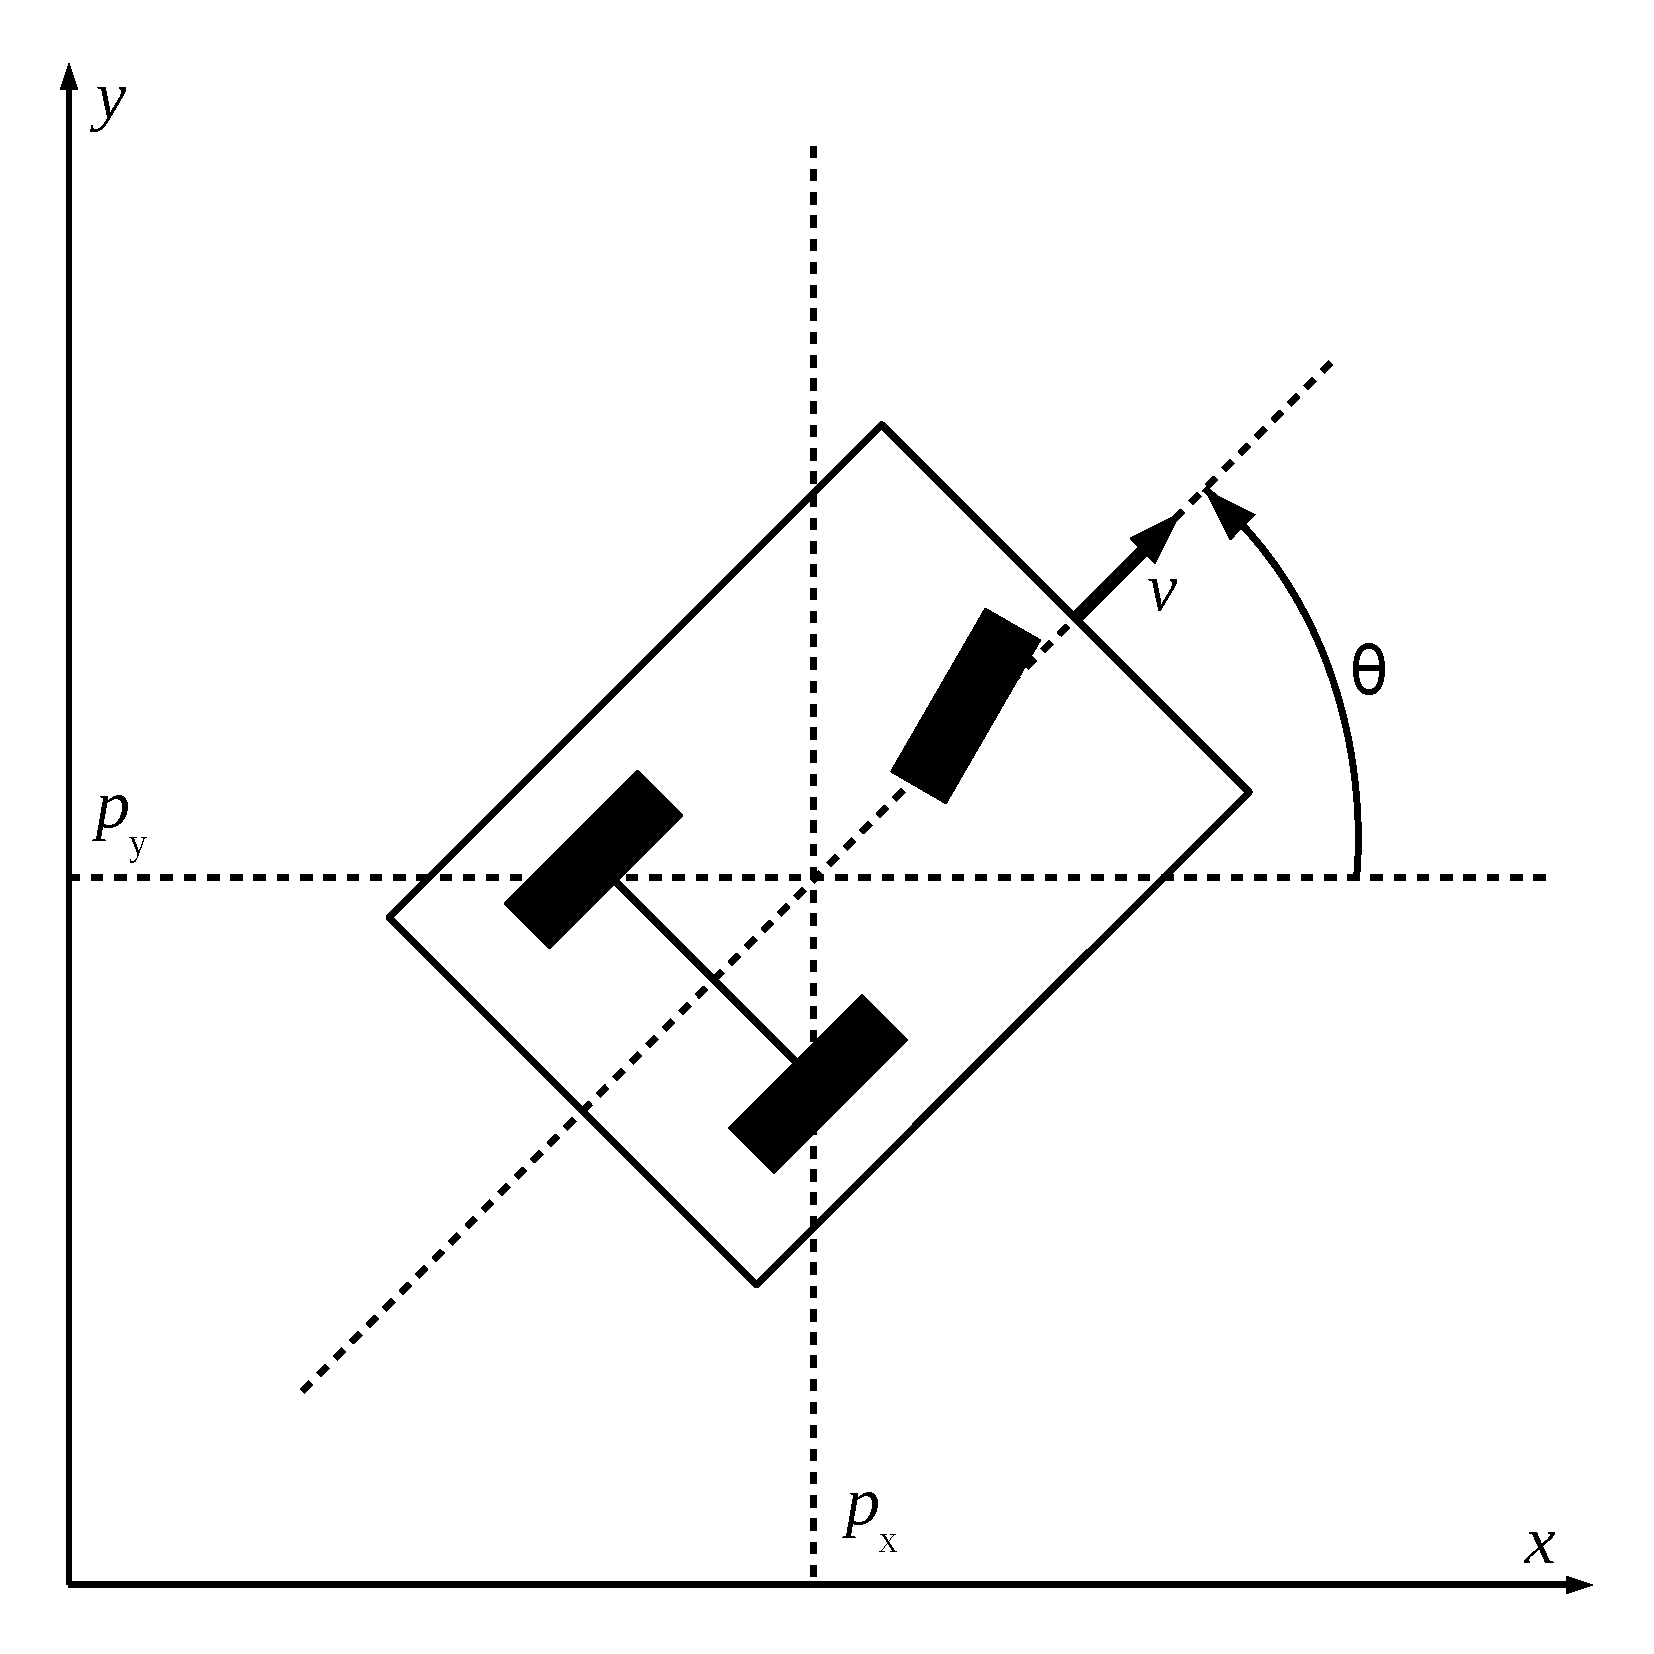
\includegraphics[width=0.4\textwidth]{Imagens/Nonholomonic-robot.pdf}
	\caption[Nonholomonic robot system representation]{Nonholomonic robot system representation. The system states $p_\textrm{x}$, $p_\textrm{y}$, $v$ and $\theta$ are highlighted.}
	\label{fig:robot}
\end{figure} 

The system described by (~\ref{eq:sistema}) is discretized by a fourth order Runge-Kutta method as described in Section~\ref{sec:discretization} and the discrete state vector $x_i$ is given by $x_i \overset{\Delta}{=} [p_{\textrm{x},i}\ \  p_{\textrm{y},i}\ \  \theta_i\ \  v_i]^T$, where subscript $i$ indicate discrete instants $iT$.

The observation model $y(t_k) \in \mathbb{R}^2$

\begin{equation}
y(t_k) = 
\begin{bmatrix}
p_\textrm{x}(t_k) \\
p_\textrm{y}(t_k)
\end{bmatrix}+v(t_k), \\
\end{equation}

\noindent
is given by the position coordinates, and $\rho(v(t_k)) = \mathcal{N} (0,R_{t_k})$ is the observation noise PDF, with zero mean and covariance $R_{t_k}$. Discrete time instants with $t_k$ are determined by random time intervals $h_k$, that is $t_{k+1}=t_k+h_k$. When time-stamp information about $t_k$ is not available, the observation vector is approximated by $\tilde{y}_i \approx y(t_k)$, where $i$ is the index of the next time instant, multiple of $T$.

Input vector $u_i = [\omega_i\ \ a_i]^T$ is measured by a girometer and accelerometer, respectively. We assume that 

\begin{equation}\label{eq:entrada}
u_i = \tilde{u}_i - w_i,
\end{equation}

\noindent
where $\tilde{u}$ represent the sensors' measured values and $\rho(w_i) = \mathcal{N} (0, Q_i)$ is the corresponding noise PDF, with zero mean and covariance $Q_i$. 

We simulate 60 seconds of robot movement, considering a step size of $\delta t_{\textrm{sim}} = 10^{-4}$. Input signals are generated arbitrarily according to Figure~\ref{fig:entrada}. 

Accuracy metrics for the unicycle position system is a modification of the RMSE defined in (\ref{eq:rmse}), to reflect error in $xy$-plane position, given by:

\begin{equation}\label{eq:pos_rmse}
RMSE_{\textrm{position}} = \frac{ \sum_{i=1}^N \sqrt{(\hat{p}_{\textrm{x},i}-p_{\textrm{x},i})^2+(\hat{p}_{\textrm{y},i}-p_{\textrm{y},i})^2}}{N},
\end{equation}

\noindent
where $\hat{p}_{\textrm{x},i}$ and $\hat{p}_{\textrm{y},i}$ are position estimates at regularly spaced time intervals $T$, $p_{\textrm{x},i}$ and $p_{\textrm{y},i}$ are true position coordinates of the unicycle, at the same time instants and $N$ is the total amount of estimates.


%sampling time intervals $h_k$ are simulated by the exponential probability distribution function from Matlab\texttrademark \ and approximated to the nearest discrete time instant, from the 600,000 available samples. 


\subsection{Unicycle Position System}

Figure~\ref{fig:exukf} shows the robot trajectory on the $xy$-plane for the given input signals, leaving from point $(0,0)$, as well as a realization of noisy and aperiodic measurements as red dots, with signal-to-noise ratio of $\textrm{SNR\textsubscript{y}} = 30$ dB and $\lambda=3.33$ Hz. Dashed blue line represents UKF estimation, considering time-stamp, $\alpha=5$ and $\textrm{SNR\textsubscript{u}} = 10 \textrm{ dB}$. 

\begin{figure}[!htb]
	\centering
	\subfigure{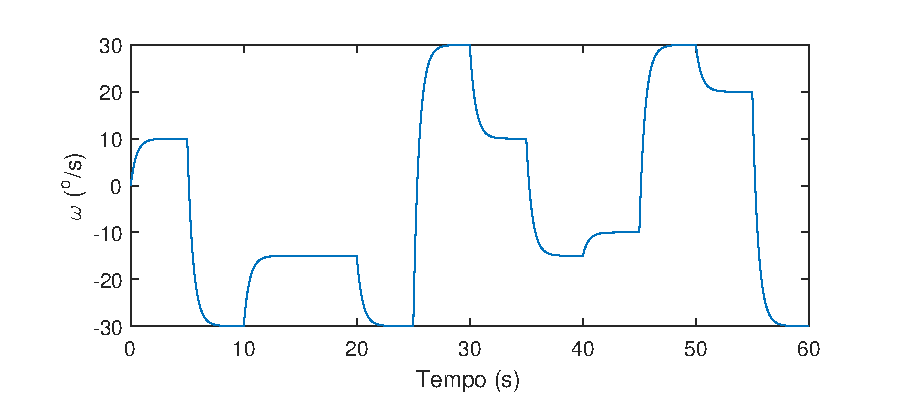
\includegraphics[width=0.8\textwidth]{Imagens/entradas1.eps}} \\
	\subfigure{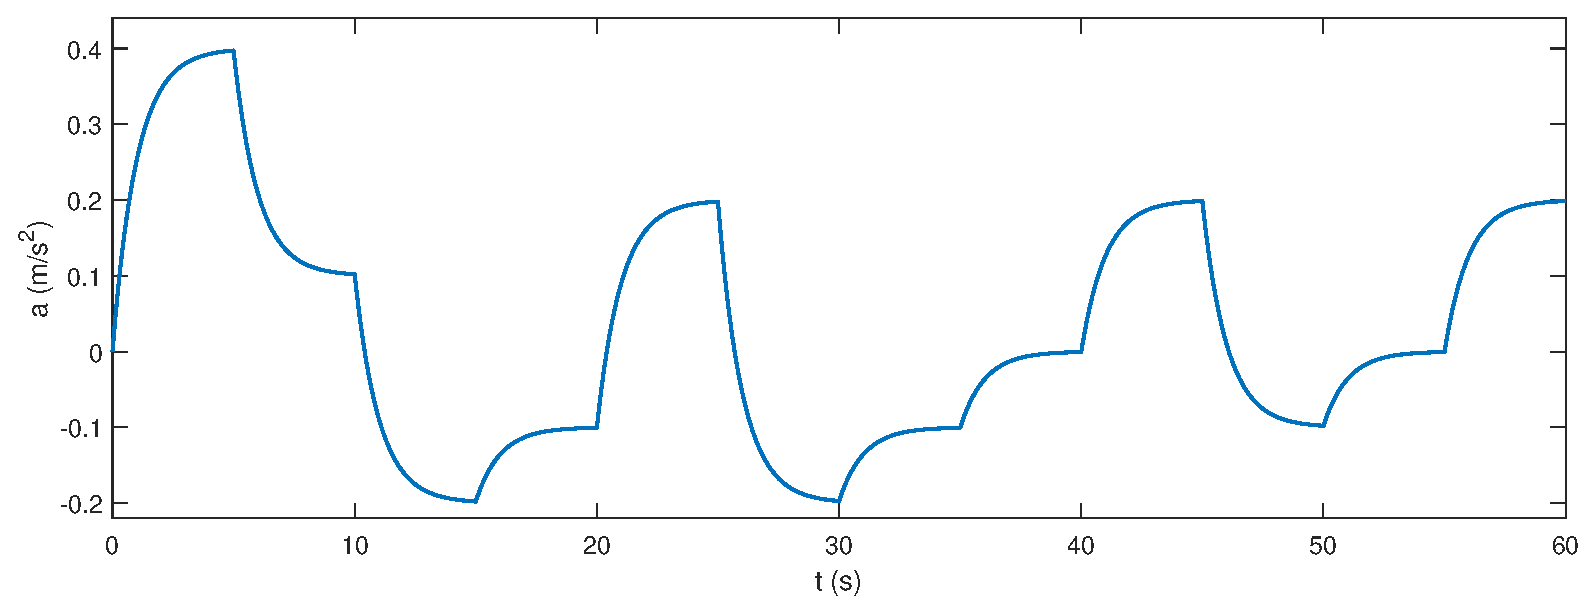
\includegraphics[width=0.8\textwidth]{Imagens/entradas2.eps}}  
	\caption[Simulation input signals]{Simulation input signals. (a) shows temporal sequence of angular velocity $\omega$ and (b) shows linear acceleration $a$.}
	\label{fig:entrada}
\end{figure}



\begin{figure}[!htb]
	\centering
	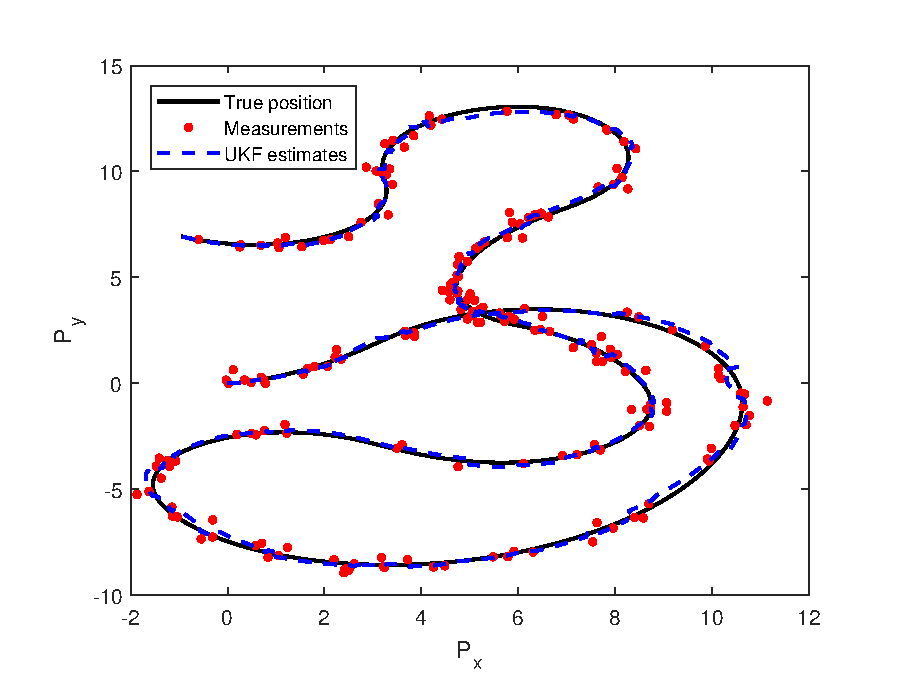
\includegraphics[width=0.7\textwidth]{Imagens/exemplo_03_30db_desloc.eps}
	\caption[True position, noisy measurements and UKF estimates]{True position (\textcolor{black}{---}), noisy measurements (\textcolor{red}{$\cdot$}) and UKF estimates (\textcolor{blue}{- -}) considering time-stamp, for a measurement noise of SNR\textsubscript{y} $= 30$ dB, $\lambda=0.3$ s and $\alpha=5$.}
	\label{fig:exukf}
\end{figure} 

Figure~\ref{fig:realizacaoJ} shows a timespan from $0$ to $1.5$ seconds of a realization of position RMSE, considering $\lambda=0.5$, $\alpha=2$, $\textrm{SNR\textsubscript{y}} = 40 \textrm{ dB}$ and $\textrm{SNR\textsubscript{u}} = 20 \textrm{ dB}$, for the UKF considering and not considering time-stamp. Black dots represent the regular time instants $kT$ whereas the asterisks on $x$-axis and dashed vertical lines match the exact measurement instants $t_k$. The first two measurements, before 0.25 seconds, are very close to the first regular time instant $1T = 0.25 \textrm{ s}$ and thus cause no significant difference on performance. It is expected, since the approximation error due to $\tilde{y}_i \approx y(t_k)$ is irrelevant. Next measurement $t_3$, taking place around $0.8$ seconds, when assimilated correctly reduces the estimate error at the correct instant. When assimilated at the next estimation time instant, the position error is not decreased appropriately. At $t_4$, around $1.1$ seconds, we can see another effect of assimilating the measurement at the correct time, with the red line decreasing slightly. 

\begin{figure}[!htb]
	\centering
	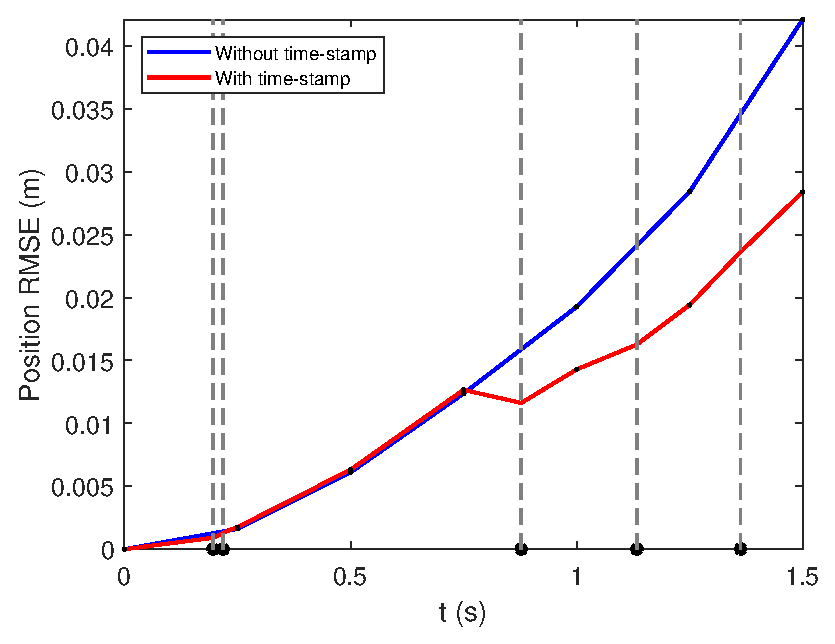
\includegraphics[width=0.7\textwidth]{Imagens/RobotJEvolution.eps}
	\caption[Performance index temporal cut for one realization]{Temporal cut from 0 to 1.5 seconds, for a realization of $J$ of both estimators, with and without time-stamp. Asterisks on $x$ axis and vertical dashed lines match the measurement sampling instants $t_k$. Black dots represent the regular estimation instants, same as input regular sampling instants.}
	\label{fig:realizacaoJ}
\end{figure} 

In the next sections we perform Monte Carlo simulations, with 1000 runs per combination of parameters, for the scenarios from Section~\ref{sec:scenarios}. Simulation parameters used for the nonlinear system are shown in Table~\ref{tab:params_robot}. For all cases, input SNR is constant at $20$ dB. All results are comprised in Figure~\ref{fig:robot_sim}, with the evolution of mean values in solid lines and the corresponding $95\%$ confidence interval in dashed lines. First row of graphs shows accuracy results for position RMSE, as described in (\ref{eq:pos_rmse}). Second and third rows present the consistency results for NEES and NIS tests, respectively, as described in Section~\ref{sec:metrics}. The blue lines are for the algorithm that considers time-stamp and red lines are for the one without time-stamp.

\begin{table}[!ht]
	\centering
	\setlength{\tabcolsep}{12pt}
	\caption[Nonlinear system simulation parameters for SNR variation]{Unicycle position estimation simulation parameters for observation SNR variation}
	\renewcommand{\arraystretch}{1.5}
	\small
	\begin{tabular}{c | c | c | c}
		\toprule
		Scenario 		& SNR observations (dB)	& $\lambda$ (Hz) & $\alpha$ \\
		\midrule
		SNR variation 	& $[100, \ 80,\ 60,\ 40,\ 20,\ 10]$ &  $10$ & $2$  \\
		$\lambda$ variation		&	$40$ & 	 $[10, \ 5,\ 0.33,\ 2.5,\ 2,\ 1.67]$ & $2$  \\
		$\alpha$ variation	&$40$ 				&  $10$ & $[10, \ 5,\ 2,\ 1]$  \\
		\bottomrule
	\end{tabular}
	\label{tab:params_robot}
\end{table}


%\begin{figure}[!htb]
%	\centering
%	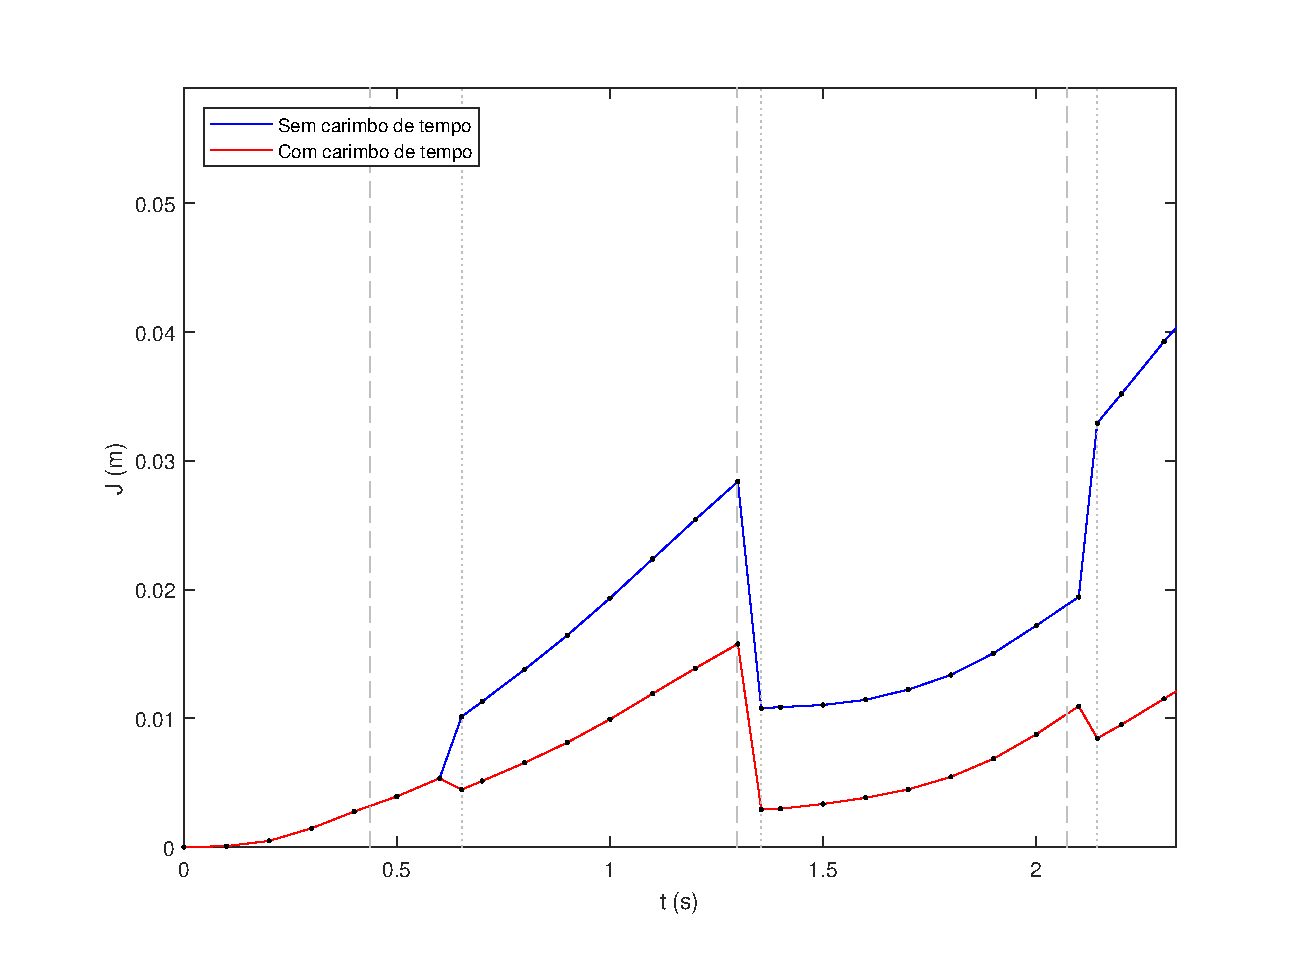
\includegraphics[width=0.8\textwidth]{Imagens/J_umarealizacao-timedelay.eps}
%%%	\caption[entrada]{Recorte temporal de 1 a 1.3 segundo, do �ndice J de uma realiza��o dos dois estimadores, com e sem carimbo de tempo. Os asteriscos no eixo $x$ representam os instantes de amostragem das observa��es $t_k$. Os pontos pretos apresentados nas linhas representam os instantes de tempo regulares de amostragem da entrada}
%	\label{fig:realizacaoJ2}
%\end{figure} 



%\setlength{\abovedisplayskip}{0.5pt}
%
%\begin{equation}\label{eq:sistema}
%\begin{split}
%\dot{\delta_e} & = -\tau^{-1},\\
%\dot{W} & = Z_{de}\delta_e + Z_wW + S_0q,\\
%\dot{q}  & = S_1 \delta_e + S_2 W + S_3q,\\
%\end{split}
%\end{equation}
%\noindent

\subsection{Measurement Signal-to-Noise Ratio Variation}\label{sec:ruido-robo}

%In this subsection we compare the estimation performance impact of considering time-stamp in the algorithm, by varying the measurement noise level. The signal-to-noise ratio for the input sensors, the measurement average time interval and $\alpha$ are held constant. Table~\ref{tab:params_robot_snr} shows the parameters used in simulation.

%\begin{table}[!ht]
%	\centering
%	\setlength{\tabcolsep}{12pt}
%	\caption[Nonlinear system simulation parameters for SNR variation]{Unicycle position estimation simulation parameters for observation SNR variation}
%	\begin{tabular}{c | c | c | c }
%		\toprule
%		SNR observations (dB)	& SNR input (dB) & $\lambda$ (Hz) & $\alpha$ \\
%		\midrule
%		$[100, \ 80,\ 60,\ 40,\ 20,\ 10]$ & $20$ & $10$ & $2$  \\
%		\bottomrule
%	\end{tabular}
%	\label{tab:params_robot_snr}
%\end{table}



% \begin{figure}[!htb]
%	\centering
%	\subfigure[]{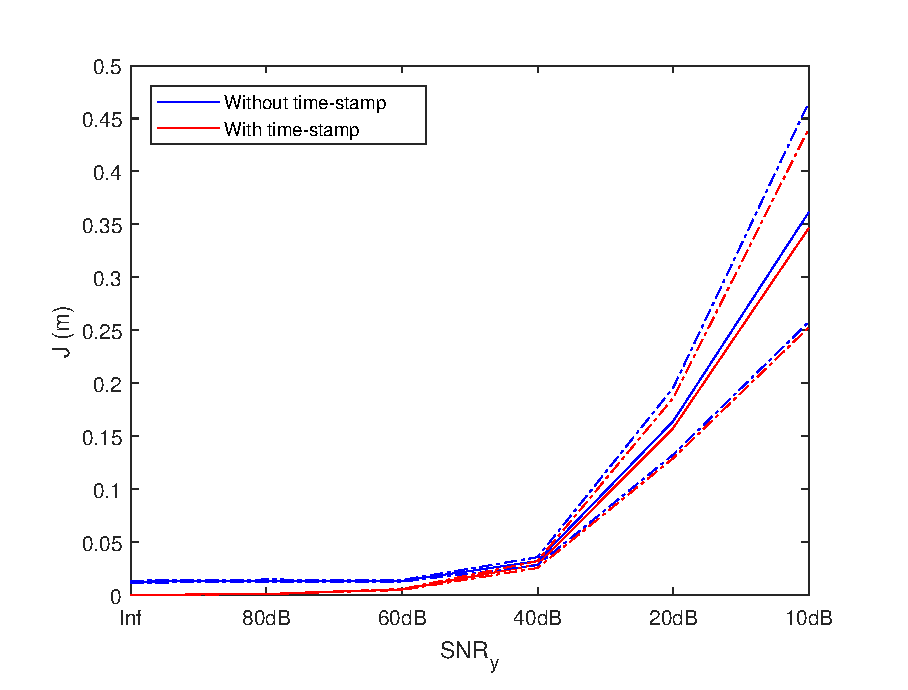
\includegraphics[width=0.49\textwidth]{Imagens/noise.eps}} 
%	\subfigure[]{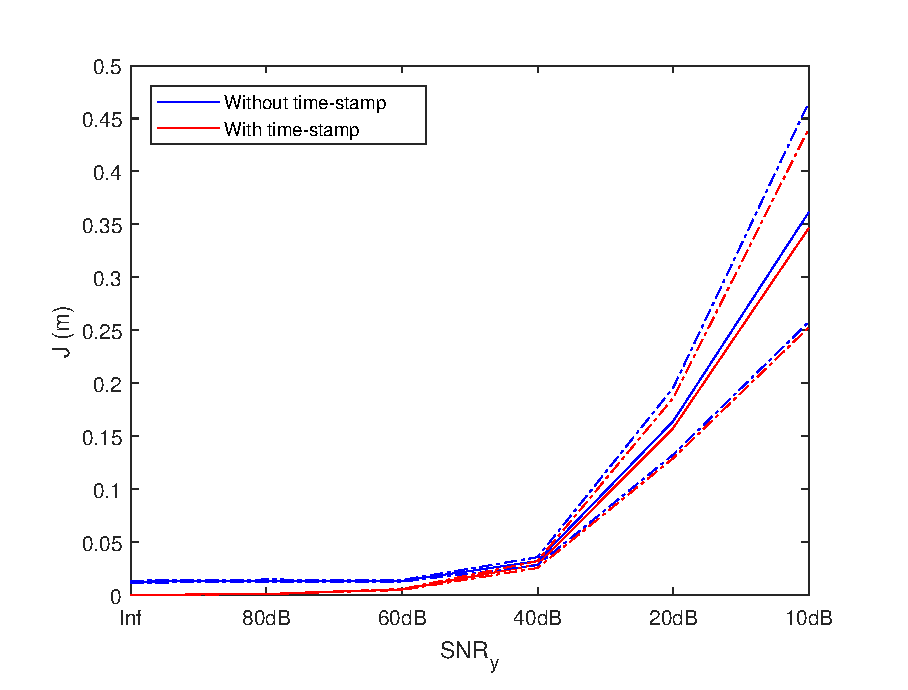
\includegraphics[width=0.49\textwidth]{Imagens/noise.eps}}  \\
%	\subfigure[]{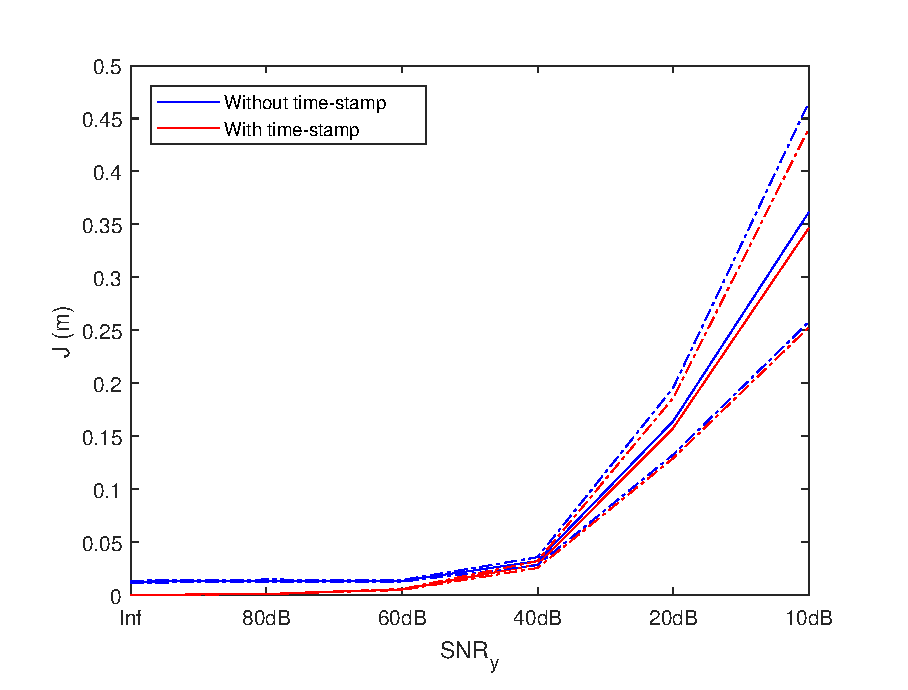
\includegraphics[width=0.49\textwidth]{Imagens/noise.eps}} 
%	\subfigure[]{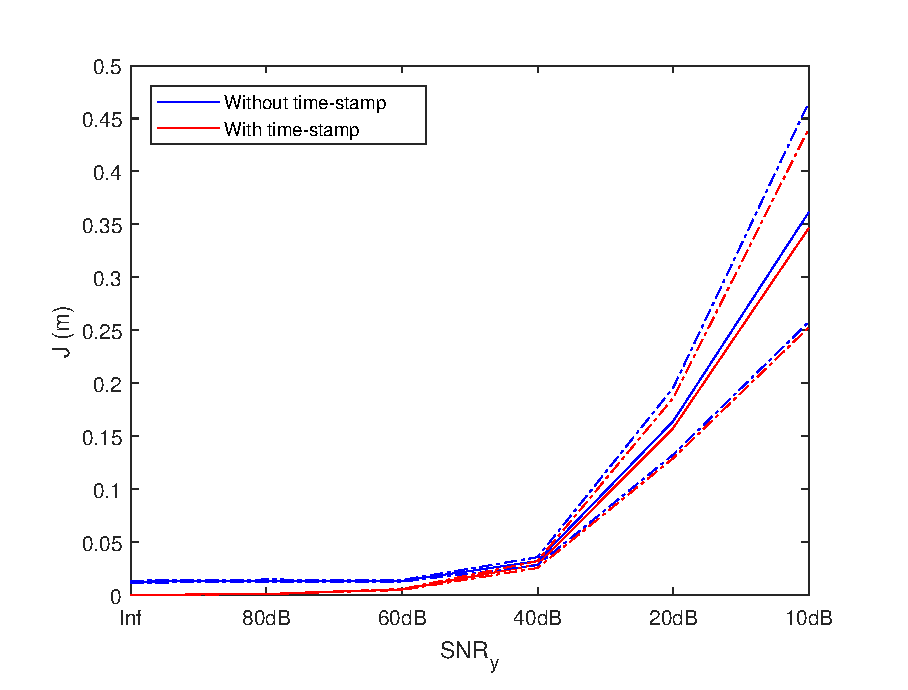
\includegraphics[width=0.49\textwidth]{Imagens/noise.eps}}     
%
%	\caption[Robot tracking performance, as a function of measurement noise]{Robot tracking performance indices with $95\%$ confidence intervals, as a function of measurement noise, for both UKF algorithms considering (\textcolor{red}{---}) and not considering (\textcolor{blue}{---}) time-stamp. Accuracy values for states $P_{\textrm{x}}$ and  $P_{\textrm{y}}$ are shown in (a) and (b), respectively. Consistency results are in (c) and (d) for NEES and NIS tests, respectively.}
%	\label{fig:robot_noise}
%\end{figure}

Results from the first column of Figure~\ref{fig:robot_sim} show the variation in performance indices for the different measurement SNR levels simulated. Both algorithms have their estimate error increased, when measurement data is contaminated with higher noise levels, as expected. It is interesting to observe, however, that the mean values are clearly different when there is less noise, in favor of considering timestamp in the estimation process. As SNR is decreased to $20$ and $10$ dB, however, both RMSE have no statistical difference. It can be explained similarly to what was observed in the linear system. The higher the noise, the more relevant are the approximation errors of $\tilde{y}_i \approx y(t_k)$. When measurements are highly contaminated with noise, these approximation errors get irrelevant for the estimation process, and both algorithms perform similarly.

Same behavior can be observed in the consistency tests results. Estimates are inconsistent for the algorithm without timestamp only for higher SNR. When noise levels increase, both algorithms have similar consistency results. Graph (g) shows a slight inconsistency in the estimation of the algorithm with timestamp, for $100$ db SNR. It is probably due to numerical errors caused by very small numbers for measurement covariances, when there is virtually no noise in data.
 

\subsection{Average Sampling Rate Variation}\label{sec:lambda-robot}

%We now consider the variation of the average sampling rate that observations are taken, maintaining the other parameters constant, according to Table~\ref{tab:params_robot_lambda}. Results for accuracy and consistency are shown in column (b) of .
%%
%\begin{table}[!ht]
%	\centering
%	\setlength{\tabcolsep}{12pt}
%	\caption[Nonlinear system simulation parameters for $\lambda$ variation]{Unicycle position estimation simulation parameters for observation $\lambda$ variation}
%	\begin{tabular}{c | c | c | c }
%		\toprule
%		SNR observations (dB)	& SNR input (dB) & $\lambda$ (Hz) & $\alpha$ \\
%		\midrule
%		$40$ 				& $20$ 		& $[10, \ 5,\ 0.33,\ 2.5,\ 2,\ 1.67]$ & $2$  \\
%		\bottomrule
%	\end{tabular}
%	\label{tab:params_robot_lambda}
%\end{table}


%\begin{figure}[!htb]
%	\centering
%	\subfigure[]{\includegraphics[width=0.49\textwidth]{Imagens/samp.eps}} 
%	\subfigure[]{\includegraphics[width=0.49\textwidth]{Imagens/samp.eps}}  \\
%	\subfigure[]{\includegraphics[width=0.49\textwidth]{Imagens/samp.eps}} 
%	\subfigure[]{\includegraphics[width=0.49\textwidth]{Imagens/samp.eps}}   
%	\caption[Robot tracking performance, as a function of measurement noise]{Robot tracking performance indices with $95\%$ confidence intervals, as a function of $\lambda$, for both UKF algorithms considering (\textcolor{red}{---}) and not considering (\textcolor{blue}{---}) time-stamp. Accuracy values for states $P_{\textrm{x}}$ and  $P_{\textrm{y}}$ are shown in (a) and (b), respectively. Consistency results are in (c) and (d) for NEES and NIS tests, respectively.}
%
%	\label{fig:samp}
%\end{figure}

As for different $\lambda$ values, variation of indices is presented in the second column of Figure~\ref{fig:robot_sim}. RMSE results suggest a slightly higher performance degradation for more sparse time intervals, providing that dynamics and other parameters are kept constant. Estimate errors seem to increase faster for the algorithm without timestamp, due to higher approximation errors of $\tilde{y}(i) \approx y(t_k)$. Another source of accuracy deterioration is the discretization error, higher for more sparse time intervals.

NEES and NIS test results suggest that both algorithms produce estimates with similar consistency levels. The reason why higher differences are not observed may derived from the use of UKF, that does not propagate error covariances, but construct them at every estimation step. 

\subsection{Regular and Average Irregular Time Interval Relation Variation}\label{sec:alpha-robot}

%We also analyze the performance impact of varying the parameter $\alpha$, which is the relation between regular input time interval $T$ and average measurements time interval $\lambda^{-1}$. Table~\ref{tab:params_robot_alpha} presets the used values for simulation and results are presented in column (c) of Table~\ref{tab:params_robot_alpha}. Results for accuracy and consistency are shown in column (b) of }.

%
%\begin{table}[!ht]
%	\centering
%	\setlength{\tabcolsep}{12pt}
%	\caption[Nonlinear system simulation parameters for $\alpha$ variation]{Unicycle position estimation simulation parameters for observation $\alpha$ variation}
%	\begin{tabular}{c | c | c | c }
%		\toprule
%		SNR observations (dB)	& SNR input (dB) & $\lambda$ (Hz) & $\alpha$ \\
%		\midrule
%		$40$ 				& $20$ 		& $10$ & $[10, \ 5,\ 2,\ 1]$  \\
%		\bottomrule
%	\end{tabular}
%	\label{tab:params_robot_alpha}
%\end{table}


%\begin{figure}[!htb]
%	\centering
%	\subfigure[]{\includegraphics[width=0.49\textwidth]{Imagens/dtudty.eps}} 
%	\subfigure[]{\includegraphics[width=0.49\textwidth]{Imagens/dtudty.eps}} \\
%	\subfigure[]{\includegraphics[width=0.49\textwidth]{Imagens/dtudty.eps}} 
%	\subfigure[]{\includegraphics[width=0.49\textwidth]{Imagens/dtudty.eps}}   
%
%	\caption[Robot tracking performance, as a function of measurement noise]{Robot tracking performance indices with $95\%$ confidence intervals, as a function of $\alpha$, for both UKF algorithms considering (\textcolor{red}{---}) and not considering (\textcolor{blue}{---}) time-stamp. Accuracy values for states $P_{\textrm{x}}$ and  $P_{\textrm{y}}$ are shown in (a) and (b), respectively. Consistency results are in (c) and (d) for NEES and NIS tests, respectively.}
%
%	\label{fig:dtudty}
%\end{figure}
Finally, the last scenario results are shown in the third column of Figure~\ref{fig:robot_sim}. They suggest that estimation performance difference is only significant for higher $\alpha$ values. Both consistency and accuracy results are similar for $\alpha =[2,1]$, when estimation is performed considering and not considering timestamp. 

For the accuracy metric, we observe an opposite trend for the nonlinear system in comparison to the linear system. Whereas estimate errors increased for higher $\alpha$ values in the linear case, here they decrease. We note that the former simulation considered SNR of $30$ dB for both measurements and input signals. In this case, however, SNR for measurements are considered to be higher than for input data, $40$ dB and $20$ dB, respectively. Therefore, the nonlinear state estimation has a higher confidence in the observation model. And, since reducing $\alpha$ values result in less sparse time intervals of observations, in comparison to input time interval, the data assimilation step is performed more frequently and increases estimation accuracy.

We also observe that the results from the algorithm with timestamp remained approximately constant throughout all cases. It indicates that when exact time instants $t_k$ are available to the estimator, the ratio given by $\alpha$ has no impact in performance. If they are not available, however, estimate errors can be multiplied by 4, if $\alpha$ varies from $1$ to $10$. 

%Such phenomenon can be explained by the fact that higher $\alpha$ values lead to smaller time steps used in the process model discretization in comparison to the measurement time intervals. Thus, approximation error originated from $\tilde{y}(i) \approx y(t_k)$ is reduced.

 \begin{figure}[!htb]
	\centering
	\subfigure[SNR variation]{\includegraphics[width=0.32\textwidth]{Imagens/robotNoise_rmse.eps}} 
	\subfigure[$\lambda$ variation]{\includegraphics[width=0.32\textwidth]{Imagens/robotSamp_rmse.eps}}  
	\subfigure[$\alpha$ variation]{\includegraphics[width=0.32\textwidth]{Imagens/robotUsamp_rmse.eps}} \\
	\subfigure[SNR variation]{\includegraphics[width=0.32\textwidth]{Imagens/robotNoise_NEES.eps}} 
	\subfigure[$\lambda$ variation]{\includegraphics[width=0.32\textwidth]{Imagens/robotSamp_NEES.eps}}  
	\subfigure[$\alpha$ variation]{\includegraphics[width=0.32\textwidth]{Imagens/robotUsamp_NEES.eps}} \\
	\subfigure[SNR variation]{\includegraphics[width=0.32\textwidth]{Imagens/robotNoise_NIS.eps}} 
	\subfigure[$\lambda$ variation]{\includegraphics[width=0.32\textwidth]{Imagens/robotSamp_NIS.eps}}  
	\subfigure[$\alpha$ variation]{\includegraphics[width=0.32\textwidth]{Imagens/robotUsamp_NIS.eps}} \\
	\caption[Nonlinear system estimation performance comparison]{Nonlinear system estimation performance indices with $95\%$ confidence intervals, as a function of SNR (a,d,g), $\lambda$ (b,e,h) and $\alpha$ (c,f,i), for algorithms with (\textcolor{red}{---}) and without (\textcolor{blue}{---}) time-stamp. Position RMSE results are shown in the first row. Consistency results are in second (NEES)) and third (NIS) rows. Horizontal gray dashed lines represent the $5\%$ significance level for the consistency tests}
	\label{fig:robot_sim}
\end{figure}


\section{Simulated Results Discussion}

Two different system are simulated to address the effects of neglecting timestamp in state estimation performance: a linear fourth order system, with two underdamped modes; and a nonlinear unicycle position system. We design three scenarios in which only one parameter of interest is changed per scenario, while the others are kept constant. That way, we can infer the contribution to performance variation to each of the parameter: SNR; $\lambda$; and $\alpha$.

For both systems, performance metrics obtained by neglecting time-stamp had a higher variability in most of the simulations, which is by itself a drawback of not considering timestamp. It indicates that that estimate accuracy and consistency are less reliable in such cases. 

The average performance metrics for the algorithm considering time-stamp were always higher or equal to the metrics from the algorithm without time-stamp, as expected. Accuracy performance for SNR variation suggested that for lower noise levels or higher SNR, the relevancy of considering or neglecting time-stamp is much higher. As noise levels increase, performance for both algorithms tend to approximate. In both cases, the lowest SNR simulated produced RMSE results that are statistically indistinguishable. 

For different $\lambda$ values, the algorithm that considers time-stamp maintained its performance metrics almost constant, specially for consistency tests, as it was expected. Results from the algorithm without timestamp indicates that more sparse observation time intervals deteriorate estimation performance, due to higher approximation errors. This deterioration is less significant for systems with faster dynamics, such is the case of the high-pass system, whose state estimate errors were similar for both algorithms, for different $\lambda$ values.

Finally, results from of performance behavior for the variation of $\alpha$ values show different behaviors for the linear and nonlinear system for the algorithm without timestamp. The linear case indicate an increase in state estimates RMSE, for smaller $\alpha$ values. Simulated parameters consider same SNR for both input and measurement data. So the more sparse are the observations, the higher are the approximation errors of assimilating data at incorrect time instants $t_k$, given by $\tilde{y}(i) \approx y(t_k)$. In the nonlinear case, we consider less noise in measurement, with two times higher SNR, that is $SNR_{\textrm{observation}} = 40$ dB and $SNR_{\textrm{input}} = 20$. Therefore, although approximation errors of $\tilde{y}(i) \approx y(t_k)$ increase for more sparse time intervals in the observations, data assimilation steps happen more frequently, contributing to a reduction of estimate errors.


%\subsection{Average Time Delay}\label{sec:dt-robot}
%
%\todo[inline,caption={Falta variar o atraso nas medi��es}]{Ainda ter� uma se��o com a varia��o do time-delay e seu impacto no desempenho}


\clearpage
